% Options for packages loaded elsewhere
\PassOptionsToPackage{unicode}{hyperref}
\PassOptionsToPackage{hyphens}{url}
\PassOptionsToPackage{dvipsnames,svgnames*,x11names*}{xcolor}
%
\documentclass[
  12pt,
  spanish,
]{book}
\usepackage{amsmath,amssymb}
\usepackage{lmodern}
\usepackage{ifxetex,ifluatex}
\ifnum 0\ifxetex 1\fi\ifluatex 1\fi=0 % if pdftex
  \usepackage[T1]{fontenc}
  \usepackage[utf8]{inputenc}
  \usepackage{textcomp} % provide euro and other symbols
\else % if luatex or xetex
  \usepackage{unicode-math}
  \defaultfontfeatures{Scale=MatchLowercase}
  \defaultfontfeatures[\rmfamily]{Ligatures=TeX,Scale=1}
\fi
% Use upquote if available, for straight quotes in verbatim environments
\IfFileExists{upquote.sty}{\usepackage{upquote}}{}
\IfFileExists{microtype.sty}{% use microtype if available
  \usepackage[]{microtype}
  \UseMicrotypeSet[protrusion]{basicmath} % disable protrusion for tt fonts
}{}
\makeatletter
\@ifundefined{KOMAClassName}{% if non-KOMA class
  \IfFileExists{parskip.sty}{%
    \usepackage{parskip}
  }{% else
    \setlength{\parindent}{0pt}
    \setlength{\parskip}{6pt plus 2pt minus 1pt}}
}{% if KOMA class
  \KOMAoptions{parskip=half}}
\makeatother
\usepackage{xcolor}
\IfFileExists{xurl.sty}{\usepackage{xurl}}{} % add URL line breaks if available
\IfFileExists{bookmark.sty}{\usepackage{bookmark}}{\usepackage{hyperref}}
\hypersetup{
  pdfauthor={Jake Bowers, Maarten Voors, and Nahomi Ichino.   Traducido por Lily Medina},
  pdflang={es},
  colorlinks=true,
  linkcolor=Maroon,
  filecolor=Maroon,
  citecolor=Blue,
  urlcolor=Blue,
  pdfcreator={LaTeX via pandoc}}
\urlstyle{same} % disable monospaced font for URLs
\usepackage[margin=1in]{geometry}
\usepackage{color}
\usepackage{fancyvrb}
\newcommand{\VerbBar}{|}
\newcommand{\VERB}{\Verb[commandchars=\\\{\}]}
\DefineVerbatimEnvironment{Highlighting}{Verbatim}{commandchars=\\\{\}}
% Add ',fontsize=\small' for more characters per line
\usepackage{framed}
\definecolor{shadecolor}{RGB}{248,248,248}
\newenvironment{Shaded}{\begin{snugshade}}{\end{snugshade}}
\newcommand{\AlertTok}[1]{\textcolor[rgb]{0.94,0.16,0.16}{#1}}
\newcommand{\AnnotationTok}[1]{\textcolor[rgb]{0.56,0.35,0.01}{\textbf{\textit{#1}}}}
\newcommand{\AttributeTok}[1]{\textcolor[rgb]{0.77,0.63,0.00}{#1}}
\newcommand{\BaseNTok}[1]{\textcolor[rgb]{0.00,0.00,0.81}{#1}}
\newcommand{\BuiltInTok}[1]{#1}
\newcommand{\CharTok}[1]{\textcolor[rgb]{0.31,0.60,0.02}{#1}}
\newcommand{\CommentTok}[1]{\textcolor[rgb]{0.56,0.35,0.01}{\textit{#1}}}
\newcommand{\CommentVarTok}[1]{\textcolor[rgb]{0.56,0.35,0.01}{\textbf{\textit{#1}}}}
\newcommand{\ConstantTok}[1]{\textcolor[rgb]{0.00,0.00,0.00}{#1}}
\newcommand{\ControlFlowTok}[1]{\textcolor[rgb]{0.13,0.29,0.53}{\textbf{#1}}}
\newcommand{\DataTypeTok}[1]{\textcolor[rgb]{0.13,0.29,0.53}{#1}}
\newcommand{\DecValTok}[1]{\textcolor[rgb]{0.00,0.00,0.81}{#1}}
\newcommand{\DocumentationTok}[1]{\textcolor[rgb]{0.56,0.35,0.01}{\textbf{\textit{#1}}}}
\newcommand{\ErrorTok}[1]{\textcolor[rgb]{0.64,0.00,0.00}{\textbf{#1}}}
\newcommand{\ExtensionTok}[1]{#1}
\newcommand{\FloatTok}[1]{\textcolor[rgb]{0.00,0.00,0.81}{#1}}
\newcommand{\FunctionTok}[1]{\textcolor[rgb]{0.00,0.00,0.00}{#1}}
\newcommand{\ImportTok}[1]{#1}
\newcommand{\InformationTok}[1]{\textcolor[rgb]{0.56,0.35,0.01}{\textbf{\textit{#1}}}}
\newcommand{\KeywordTok}[1]{\textcolor[rgb]{0.13,0.29,0.53}{\textbf{#1}}}
\newcommand{\NormalTok}[1]{#1}
\newcommand{\OperatorTok}[1]{\textcolor[rgb]{0.81,0.36,0.00}{\textbf{#1}}}
\newcommand{\OtherTok}[1]{\textcolor[rgb]{0.56,0.35,0.01}{#1}}
\newcommand{\PreprocessorTok}[1]{\textcolor[rgb]{0.56,0.35,0.01}{\textit{#1}}}
\newcommand{\RegionMarkerTok}[1]{#1}
\newcommand{\SpecialCharTok}[1]{\textcolor[rgb]{0.00,0.00,0.00}{#1}}
\newcommand{\SpecialStringTok}[1]{\textcolor[rgb]{0.31,0.60,0.02}{#1}}
\newcommand{\StringTok}[1]{\textcolor[rgb]{0.31,0.60,0.02}{#1}}
\newcommand{\VariableTok}[1]{\textcolor[rgb]{0.00,0.00,0.00}{#1}}
\newcommand{\VerbatimStringTok}[1]{\textcolor[rgb]{0.31,0.60,0.02}{#1}}
\newcommand{\WarningTok}[1]{\textcolor[rgb]{0.56,0.35,0.01}{\textbf{\textit{#1}}}}
\usepackage{longtable,booktabs,array}
\usepackage{calc} % for calculating minipage widths
% Correct order of tables after \paragraph or \subparagraph
\usepackage{etoolbox}
\makeatletter
\patchcmd\longtable{\par}{\if@noskipsec\mbox{}\fi\par}{}{}
\makeatother
% Allow footnotes in longtable head/foot
\IfFileExists{footnotehyper.sty}{\usepackage{footnotehyper}}{\usepackage{footnote}}
\makesavenoteenv{longtable}
\usepackage{graphicx}
\makeatletter
\def\maxwidth{\ifdim\Gin@nat@width>\linewidth\linewidth\else\Gin@nat@width\fi}
\def\maxheight{\ifdim\Gin@nat@height>\textheight\textheight\else\Gin@nat@height\fi}
\makeatother
% Scale images if necessary, so that they will not overflow the page
% margins by default, and it is still possible to overwrite the defaults
% using explicit options in \includegraphics[width, height, ...]{}
\setkeys{Gin}{width=\maxwidth,height=\maxheight,keepaspectratio}
% Set default figure placement to htbp
\makeatletter
\def\fps@figure{htbp}
\makeatother
\setlength{\emergencystretch}{3em} % prevent overfull lines
\providecommand{\tightlist}{%
  \setlength{\itemsep}{0pt}\setlength{\parskip}{0pt}}
\setcounter{secnumdepth}{5}
\usepackage{booktabs}
\usepackage{amsthm}
\makeatletter
\def\thm@space@setup{%
  \thm@preskip=8pt plus 2pt minus 4pt
  \thm@postskip=\thm@preskip
}
\makeatother
%\usepackage[T1]{fontenc}
%\usepackage{textcomp}
%\usepackage{fontspec}
%\mainfont[Ligatures=TeX]{Lato}
\usepackage{polyglossia}
\setdefaultlanguage{spanish}
\usepackage{fancyhdr}
\pagestyle{fancy}
\fancyhf{}
\fancyfoot[LE,LO]{
\includegraphics[width=2cm]{Images/egap-logo.png}}
\fancyfoot[RE,RO]{\thepage}
%\usepackage{libertinus}
%\usepackage[autocite=plain,style=verbose,citetracker=false]{biblatex}
\usepackage[autocite=plain,citestyle=verbose]{biblatex}
\usepackage{caption}


\ifxetex
  % Load polyglossia as late as possible: uses bidi with RTL langages (e.g. Hebrew, Arabic)
  \usepackage{polyglossia}
  \setmainlanguage[]{spanish}
\else
  \usepackage[main=spanish]{babel}
% get rid of language-specific shorthands (see #6817):
\let\LanguageShortHands\languageshorthands
\def\languageshorthands#1{}
\fi
\ifluatex
  \usepackage{selnolig}  % disable illegal ligatures
\fi
\usepackage[]{biblatex}
\addbibresource{learningdays-book.bib}
\newlength{\cslhangindent}
\setlength{\cslhangindent}{1.5em}
\newlength{\csllabelwidth}
\setlength{\csllabelwidth}{3em}
\newenvironment{CSLReferences}[2] % #1 hanging-ident, #2 entry spacing
 {% don't indent paragraphs
  \setlength{\parindent}{0pt}
  % turn on hanging indent if param 1 is 1
  \ifodd #1 \everypar{\setlength{\hangindent}{\cslhangindent}}\ignorespaces\fi
  % set entry spacing
  \ifnum #2 > 0
  \setlength{\parskip}{#2\baselineskip}
  \fi
 }%
 {}
\usepackage{calc}
\newcommand{\CSLBlock}[1]{#1\hfill\break}
\newcommand{\CSLLeftMargin}[1]{\parbox[t]{\csllabelwidth}{#1}}
\newcommand{\CSLRightInline}[1]{\parbox[t]{\linewidth - \csllabelwidth}{#1}\break}
\newcommand{\CSLIndent}[1]{\hspace{\cslhangindent}#1}

\title{La teoría y la práctica de los experimentos de campo:\\
Una introducción de los Learning Days de EGAP}
\author{Jake Bowers,\footnote{El orden en el que aparecen los autores fue generado aleatoriamente. \url{https://jakebowers.org}} Maarten Voors,\footnote{\url{https://sites.google.com/site/maartenvoors/}} and Nahomi Ichino\footnote{\url{https://nahomi.github.io/}}. Traducido por Lily Medina\footnote{\url{https://lilymedina.github.io/}}}
\date{01-09-21}

\begin{document}
\maketitle

\captionsetup[table]{list=no}
\captionsetup[figure]{list=no}

{
\hypersetup{linkcolor=}
\setcounter{tocdepth}{1}
\tableofcontents
}
\hypertarget{introducciuxf3n}{%
\chapter{Introducción}\label{introducciuxf3n}}

A lo largo de la última decada, \href{http://egap.org/}{Evidence in Governance and Politics (EGAP)} ha organizado la serie de talleres, \href{https://egap.org/learning-days/}{Learning Days}, con el fin de generar capacidad para la investigación experimental en ciencias sociales entre investigadores principales (IP), tanto ciéntificos como profesionales expertos, en África y América Latina. Al promover el uso de métodos prácticos y estadísticos relacionados con experimentos aleatorios de campo, la iniciativa de los Learning Days busca identificar y nutrir redes de investigadores en todo el mundo y crear conexiones sólidas y productivas entre estos investigadores y los miembros de EGAP.

Los Learning Days son una combinación de clínicas de diseño, presentaciones de investigaciones, trabajo guiado usando un software estadístico y conferencias temáticas a cargo de un pequeño grupo de instructores, en su mayoría profesores y estudiantes de doctorado de la red EGAP. Los talleres se enfocan en el uso de métodos para el diseño y análisis de experimentos aleatorios de campo en lugar de experimentos aleatorios de laboratorio o estudios no aleatorios.

\textbf{Este libro} surgió del deseo de compartir el materia didáctico que hemos venido desarrollando para los Learning Days. La versión actual está dirigida a \textbf{instructores y organizadores} de talleres y cursos similares que se especialicen en formar investigadores principales tales como profesores, becarios post-doctorales, estudiantes de doctorado y evaluadores de organizaciones gubernamentales y no-gubernamentales que implementen estudios aleatorios de programas relacionados con el estudio de las instituciones, la gobernanza y el desarrollo. Gran parte del material didáctico también le será útil a los participantes de sesiones pasadas de los Learning Days.

Este libro presenta una extensa reseña de métodos basados en inferencia causal para investigadores que están desarrollando algún diseño de investigación experimental. El libro está organizado en \textbf{módulos} y cubre temas como inferencia causal, aleatorización, pruebas de hipótesis, estimaciones, estimadores, poder estadístico, medición, amenazas a la validez interna y ética de experimentos. Los módulos aparecen en el orden que los instructores de los Learning Days han considerado más útil. Sin embargo, dado que los módulos están relacionados entre sí, pueden reordenarse para adaptarse a sus necesidades como instructor. En el apéndice, incluimos algunos preliminares del curso, como por ejemplo un \href{glosario-de-términos.html}{glosario de términos} y \href{introducción-a-r-y-rstudio.html}{una introducción a R y RStudio}.

El libro también incluye \textbf{diapositivas} con el contenido principal, un \href{researchdesignform.html}{formulario de diseño de investigación de EGAP} y \textbf{referencias} a algunos ejemplos de estudios de investigación y diapositivas empleadas en sesiones pasadas de los Learning Days. Este material conecta con y está basado en el trabajo resumido en \href{https://egap.org/methods-guides/}{las guías de métodos de EGAP}. Hemos ampliado el material proveniente de sesiones pasados de los Learning Days sobre pruebas de hipótesis, estimación y poder estadístico y hemos agregado nuevos módulos sobre el proceso de diseño de investigación, medición y consideraciones éticas. Las diapositivas y los módulos que se presentan a continuación contienen demasiada información para que sea cubierta en una sola semana (la duración habitual de un taller de Learning Days). Sin embargo hemos decidido incluir más información en lugar de menos para ayudar a los instructores a adaptar sus cursos a sus audiencias específicas.

\hypertarget{cuxf3mo-usar-este-libro}{%
\section{Cómo usar este libro}\label{cuxf3mo-usar-este-libro}}

Para que pueda obtener el mayor beneficio de este libro, le recomendamos tener \href{https://cran.r-project.org/}{R} y \href{https://www.rstudio.com/products/rstudio/download/}{RStudio} instalados en su computador. De hecho, en las diapositivas se asume que usted utilizará R markdown para adaptarlas a sus propios fines.

Para familiarizarse con R, le recomendamos consultar el módulo \href{introducción-a-r-y-rstudio.html}{Introducción a R y R Studio}.

Si desea puede copiar este libro o partes del mismo (por ejemplo, diapositivas, etc.) usando el botón para Descargar (Download) en la página principal de \url{http://github.com/egap/theory_and_practice_of_field_experiments} o directamente en GitHub bifurcando (forking) este repositorio.

Cualquier persona puede utilizar el material didáctico, siempre y cuando se le reconozca al autor y se dé crédito a EGAP. Por favor, consulte la licencia internacional Creative Commons Attribution-ShareAlike 4.0 para conocer los términos exactos.

\hypertarget{nos-encantaruxeda-saber-lo-que-piensa}{%
\section{¡Nos encantaría saber lo que piensa!}\label{nos-encantaruxeda-saber-lo-que-piensa}}

Si tiene alguna pregunta, comentario o ha organizado su propio evento, ¡póngase en contacto con nosotros! Para hacerlo puede crear un \emph{issue} en \href{https://github.com/egap/theory_and_practice_of_field_experiments/issues}{Github} o escríbirnos sus comentarios usando hypothes.is en su navegador. Por favor escríbanos al correo electrónico \href{mailto:admin@egap.org}{\nolinkurl{admin@egap.org}} con sus comentarios. Estaremos revisando dicha cuenta periódicamente.

\hypertarget{agradecimientos}{%
\section{Agradecimientos}\label{agradecimientos}}

Los materiales incluidos en este libro han sido desarrollados a lo largo de los últimos años por distintos instructores que han participado en los Learning Days. Entre estos se encuentran (presentados en orden alfabético): Jake Bowers, Jasper Cooper, Ana De la O, Lindsay Dolan, Natalia Garbiras Díaz, Macartan Humphreys, Nahomi Ichino, Salif Jaiteh, Gareth Nellis, Dan Nielson, Rafael Piñeiro, Fernando Rosenblatt, Tara Slough, Peter van der Windt y Maarten Voors. Queremos agradecer especialmente a Natalia Garbiras Díaz, Macartan Humphreys, Anghella Brigeth Rosero Rodríguez y Tara Slough por sus comentarios a un borrador inicial de este libro.

En EGAP, Matt Lisiecki, Ingrid Lee, Goldie Negelev, Max Mendez-Beck y otros han brindado un apoyo extraordinario. Los Learning Days han sido generosamente financiados por la Fundación Hewlett y apoyados por instituciones en todo el mundo, entre ellas la Escuela Africana de Economía (Benin), la Universidad Diego Portales (Chile), la Universidad de los Andes (Colombia), el Centro de Ghana para el Desarrollo Democrático (Ghana), Mercy Corps (Guatemala), Invest in Knowledge (Malawi), NYU Abu Dhabi (EAU) y la Universidad Católica del Uruguay (Uruguay).

\hypertarget{el-proceso-del-diseuxf1o-de-investigaciuxf3n}{%
\chapter{El Proceso del diseño de investigación}\label{el-proceso-del-diseuxf1o-de-investigaciuxf3n}}

Este libro tiene como propósito ayudarle a comprender y a diseñar experimentos aleatorios de campo. Pero antes de sumergirnos en los detalles del diseño de una investigación, lo primero que necesitamos es una pregunta de investigación bien formulada, una pregunta que nos permita generar conocimiento o nos ayude a tomar decisiones relacionadas con políticas públicas. O ambas cosas. Para esto no hay una receta simple, pero nuestras teorías sobre cómo funciona el mundo son importantes para poder articular bien las preguntas que serán la base de una investigación de alto impacto. Lo que sigue después de formular nuestra pregunta es desarrollar el mejor diseño experimental posible de acuerdo a nuestros recursos, utilizando el conocimiento de inferencia causal y estadística proveniente de los módulos que vienen a continuación.

Este módulo presenta el \href{https://egap.github.io/learningdays-resources/Exercises/design-form.Rmd}{formulario para el diseño de investigación de EGAP}, una lista de verificación que le servirá de guia a través de las muchas etapas del proceso de investigación. Los talleres de los Learning Days se organizan en torno a este formulario. También le recomendamos el uso del paquete de software \href{http://declaredesign.org}{DeclareDesign} para explorar las implicaciones que podrían tener las diferentes elecciones que se pueden tomar con respecto al diseño de la investigación. Finalmente, este módulo discute los planes de pre-análisis y pre-registro. Cuando planificamos nuestros análisis y hacemos públicos estos planes, hacemos que sea más fácil persuadir a otros con nuestros resultados.

\hypertarget{contenido-principal}{%
\section{Contenido principal}\label{contenido-principal}}

\begin{itemize}
\item
  Una \textbf{pregunta de investigación bien formulada} facilita el avance de la ciencia y/o puede informar decisiones relacionadas con políticas públicas.
\item
  Ciertos \textbf{diseños de investigación} son más apropiados para abordar ciertas preguntas. La idea es elegir el diseño que mejor se ajuste a nuestras preguntas claves de acuerdo a nuestras limitaciones.
\item
  Las preguntas que hacemos surgen, a menudo de manera implícita, de nuestros valores y de nuestra forma de entender cómo funciona el mundo. Estas \textbf{teorías} hacen que nuestras preguntas sean relevantes. Los experimentos que realizamos nos enseñan acerca de estas teorías. Es decir, esperamos que la evidencia y los datos que surjan a partir de estos diseños de investigación mejoren nuestro entendimiento del mundo.
\item
  Componentes principales de un diseño de investigación.
\item
  Presentar los componentes principales del \href{https://egap.github.io/learningdays-resources/Exercises/design-form.html}{formulario para el diseño de investigación de EGAP}.
\item
  Presentar el paquete de software para diseño de investigaciones, \href{http://declaredesign.org}{DeclareDesign}.
\item
  Corriente de las ciencias sociales que está enfocada en la \textbf{revisión de diseños, en lugar de resultados}.
\item
  \textbf{Pre-registro:} qué es, por qué y cómo deberíamos hacerlo.
\end{itemize}

\hypertarget{diapositivas}{%
\section{Diapositivas}\label{diapositivas}}

A continuación presentamos las diapositivas con el contenido principal que cubrimos en nuestra clase sobre diseño de investigación. Usted puede usar directamente los archivos originales de las diapositivas o también puede copiarlos y editarlos localmente.

\begin{itemize}
\item
  \href{https://egap.github.io/learningdays-resources/Slides/researchdesignform-slides.Rmd}{Archivos de R Markdown}
\item
  \href{https://egap.github.io/learningdays-resources/Slides/researchdesignform-slides.pdf}{Versión en PDF}
\item
  \href{https://egap.github.io/learningdays-resources/Slides/researchdesignform-slides.html}{Versión de HTML}
\end{itemize}

Si desea, también puede ver las diapositivas utilizadas en sesiones previas de los Learning Days de EGAP:

\begin{itemize}
\item
  \href{https://egap.github.io/learningdays-resources/Slides/Examples/declare_design-montevideo.pdf}{Presentación de DeclareDesign de los Learning Days de EGAP en la Universidad Católica del Uruguay, Montevideo, marzo de 2018}
\item
  \href{https://egap.github.io/learningdays-resources/Slides/Examples/declare_design-malawi.pdf}{Presentación de DeclareDesign de los Learning Days de EGAP en Salima, Malawi, febrero de 2017}
\item
  \href{https://egap.github.io/learningdays-resources/Slides/Examples/declare_design-santiago.pdf}{Presentación de DeclareDesign de los Learning Days de EGAP en la Universidad Diego Portales in Santiago, Chile, mayo de 2016}
\end{itemize}

Si desea, también puede ver las diapositivas para las charlas de diseño de sesiones pasadas de los Learning Days de EGAP, donde los instructores se centran en problemas que pueden surgir mientras se diseña una investigación en vez de enfocarse en los resultados:

\begin{itemize}
\item
  \href{https://egap.github.io/learningdays-resources/Slides/Examples/research_design_2-benin.pdf}{Charla de Diseño de los Learning Days de EGAP en la Escuela Africana de Economía, Benin, marzo de 2018}
\item
  \href{https://egap.github.io/learningdays-resources/Slides/Examples/research_design_1-montevideo.pdf}{Charla de Diseño 1 de los Learning Days de EGAP en la Universidad Católica del Uruguay, Montevideo, marzo de 2018}
\item
  \href{https://egap.github.io/learningdays-resources/Slides/Examples/research_design_2-montevideo.pdf}{Charla de Diseño 2 de los Learning Days de EGAP en la Universidad Católica del Uruguay, Montevideo, marzo de 2018}
\item
  \href{https://egap.github.io/learningdays-resources/Slides/Examples/research_design_3-montevideo.pdf}{Charla de Diseño 3 de los Learning Days de EGAP en la Universidad Católica del Uruguay, Montevideo, marzo de 2018}
\item
  \href{https://egap.github.io/learningdays-resources/Slides/Examples/research_design_1-santiago.pdf}{Charla de Diseño 1 de los Learning Days de EGAP en la Universidad Diego Portales en Santiago, Chile, mayo de 2016}
\item
  \href{https://egap.github.io/learningdays-resources/Slides/Examples/research_design_2-santiago.pdf}{Charla de Diseño 2 de los Learning Days de EGAP en la Universidad Diego Portales en Santiago, Chile, mayo de 2016}
\item
  \href{https://egap.github.io/learningdays-resources/Slides/Examples/research_design_3-santiago.pdf}{Charla de Diseño 3 de los Learning Days de EGAP en la Universidad Diego Portales en Santiago, Chile, mayo de 2016}
\item
  \href{https://egap.github.io/learningdays-resources/Slides/Examples/research_design-guatemala.pdf}{Charla de Diseño de los Learning Days de EGAP en la Ciudad de Guatemala, Guatemala, agosto de 2017}
\end{itemize}

\hypertarget{formulario-de-diseuxf1o-y-pre-registro}{%
\section{Formulario de diseño y pre-registro}\label{formulario-de-diseuxf1o-y-pre-registro}}

\begin{itemize}
\item
  \href{https://egap.github.io/learningdays-resources/Exercises/design-form.html}{Formulario de diseño de investigación de EGAP}. Lista de verificación creada para los Learning Days para guiarlo a través de las etapas del proceso de investigación.

  \begin{itemize}
  \item
    \href{https://egap.github.io/learningdays-resources/Exercises/design-form.docx}{Versión Docx}
  \item
    \href{https://egap.github.io/learningdays-resources/Exercises/design-form.pdf}{Versión en PDF}
  \item
    \href{https://egap.github.io/learningdays-resources/Exercises/design-form.html}{Versión de HTML}
  \end{itemize}
\item
  Enlace a los repositorios de pre-registro/pre-análisis:

  \begin{itemize}
  \item
    Registro EGAP, alojada en OSF (\url{https://egap.org/registry/})
  \item
    Registro de AEA RCT (\url{https://www.socialscienceregistry.org/})
  \item
    OSF (\url{https://osf.io/registries})
  \end{itemize}
\item
  Ejemplos de planes de pre-registro/pre-análisis:

  \begin{itemize}
  \item
    Mensajes de Texto en Mozambique del \href{https://oes.gsa.gov/projects/sms-mozambique/}{Gobierno Federal de Estados Unidos}
  \item
    Cámaras corporales para la policia de \href{https://osf.io/472zh}{Lab DC}
  \end{itemize}
\end{itemize}

\hypertarget{recursos}{%
\section{Recursos}\label{recursos}}

\hypertarget{guuxeda-de-muxe9todos-de-egap}{%
\subsection{Guía de métodos de EGAP}\label{guuxeda-de-muxe9todos-de-egap}}

\begin{itemize}
\item
  Guía de métodos de EGAP \href{https://egap.org/resource/10-things-to-know-about-pre-analysis-plans/}{Las 10 cosas que usted debe saber sobre los planes de pre-análisis}
\item
  Guía de métodos de EGAP \href{https://egap.org/resource/10-things-to-know-about-measurement-in-experiments/}{Las 10 cosas que usted debe saber sobre medición en experimentos}
\end{itemize}

\hypertarget{libros-capuxedtulos-y-artuxedculos}{%
\subsection{Libros, capítulos y artículos}\label{libros-capuxedtulos-y-artuxedculos}}

\begin{itemize}
\item
  \href{https://oes.gsa.gov/assets/files/preregistration-as-a-tool-in-federal-evaluation.pdf}{El pre-registro como herramienta para fortalecer la evaluación federal (en Inglés)}. Un libro blanco de la oficina de ciencias de la evaluación del gobierno de los Estados Unidos. Si desea, también puede ver ejemplos de sus planes de pre-análisis en todas sus \href{https://oes.gsa.gov/work/}{páginas sobre experimentos de campo}.
\item
  \autocite{christensen_transparent_2019}. Este libro resume los nuevos enfoques de la investigación en ciencias sociales sobre transparencia y reproducibilidad.
\item
  \autocite{gerber_field_2012}. El capitulo 12 contiene algunos ejemplos de diseño de investigación experimental.
\end{itemize}

\hypertarget{herramientas}{%
\subsection{Herramientas}\label{herramientas}}

\begin{itemize}
\tightlist
\item
  \href{https://declaredesign.org/}{DeclareDesign}, un conjunto de herramientas de software para describir, evaluar y realizar investigaciones empíricas.
\end{itemize}

\hypertarget{inferencia-causal}{%
\chapter{Inferencia causal}\label{inferencia-causal}}

Gran parte del estudio de las ciencias sociales gira en torno a la causalidad. Nos hacemos preguntas del tipo: \href{https://egap.org/resource/electoral-administration-in-kenya/}{¿acaso la inscripción de los electores aumenta su participación política?}, \href{https:\%20//\%20egap.org/resource/does-bottom-up-accountability-work-evidence-from-uganda/}{¿pueden los sistemas de rendición de cuentas que parten desde las bases sociales mejorar indicadores de salud?}, o \href{https://egap.org/resource/brief\%20-70-cómo-las-narrativas-personales-reducen-las-actitudes-negativas-hacia-los-inmigrantes-en-Kenia\%20/}{¿ayudan las narrativas personales de los inmigrantes a reducir las actitudes perjudiciales hacia ellos?}.

A lo largo de la última década, el estudio de las ciencias sociales se ha vuelto mucho más riguroso al momento de hacer afirmaciones de tipo causal, basándose en una larga historia de trabajo sobre causalidad que se remonta a los escritos clásicos de \protect\hyperlink{ux5cux2520causalinference-classics}{Fisher y Rubin}. El uso de experimentos se ha vuelto cada vez más común y la aleatorización se ha convertido en la herramienta ideal para abordar temas de causalidad.

En este módulo presentamos el enfoque contrafactual de la inferencia causal y cómo se pueden interpretar las afirmaciones de tipo causal. Presentamos el marco de salidas potenciales (potential outcomes) y cómo la asignación aleatoria nos ayuda a hacer afirmaciones sobre lo que habría sucedido en ausencia de alguna política, acción o programa que estudiamos. También discutimos los tres supuestos básicos necesarios para la inferencia causal: asignación aleatoria de sujetos a tratamientos, no interferencia y excluibilidad.

\hypertarget{contenido-principal-1}{%
\section{Contenido principal}\label{contenido-principal-1}}

\begin{itemize}
\item
  ¿A qué nos referimos cuando decimos que algo es una \textbf{causa} de algo más? ¿Y por qué es importante ser claro acerca de lo que una afirmación de tipo causal quiere decir?
\item
  Una introducción al tema de \textbf{salidas potenciales} como forma para pensar en alternativas para posibles versiones del mundo.
\item
  La \textbf{aleatorización} nos ayuda a entender las afirmaciones contrafactuales de tipo causal.
\item
  Los tres \textbf{supuestos básicos} claves para la inferencia causal: asignación aleatoria de sujetos a los distintos grupos experimentales, no interferencia y posibilidad de exclusión.
\item
  Comparación de estudios aleatorizados con estudios observacionales.
\item
  La aleatorización contibruye significativamente a la validez interna, pero no necesariamente alcanza la \textbf{validez externa}.
\item
  Una pregunta causal está estrechamente relacionada con el \href{the-research-design-process.html}{diseño de la investigación}.
\end{itemize}

\hypertarget{diapositivas-1}{%
\section{Diapositivas}\label{diapositivas-1}}

A continuación presentamos las diapositivas con el contenido principal cubierto durante nuestra clase sobre causalidad. Usted puede usar directamente los archivos originales de las diapositivas o también puede copiarlos y editarlos localmente.

\begin{itemize}
\item
  \href{https://egap.github.io/learningdays-resources/Slides/causalinference-slides.Rmd}{Archivo de R Markdown}
\item
  \href{https://egap.github.io/learningdays-resources/Slides/causalinference-slides.pdf}{Versión en PDF}
\item
  \href{https://egap.github.io/learningdays-resources/Slides/causalinference-slides.html}{Versión de HTML}
\end{itemize}

Si desea, también puede ver las diapositivas utilizadas en sesiones pasadas de los Learning Days de EGAP:

\begin{itemize}
\item
  \href{https://egap.github.io/learningdays-resources/Slides/Examples/causality-benin.pdf}{Presentación sobre inferencia causal de los Learning Days de EGAP en la Escuela Africana de Economía, Abomey-Calavi, junio de 2019}
\item
  \href{https://egap.github.io/learningdays-resources/Slides/Examples/causality-bogota.pdf}{Presentación sobre inferencia causal de los Learning Days de EGAP en la Universidad de Los Andes, Bogotá, abril de 2019}
\item
  \href{https://egap.github.io/learningdays-resources/Slides/Examples/causality-montevideo.pdf}{Presentación sobre inferencia causal de los Learning Days de EGAP en la Universidad Católica del Uruguay, Montevideo, marzo de 2018}
\item
  \href{https://egap.github.io/learningdays-resources/Slides/Examples/causality-guatemala.pdf}{Presentación sobre inferencia causal de los Learning Days de EGAP en la Ciudad de Guatemala, Guatemala, agosto de 2017}
\item
  \href{https://egap.github.io/learningdays-resources/Slides/Examples/intro_experiments-guatemala.pdf}{Presentación de la clase de introducción a experimentos de los Learning Days de EGAP en la Ciudad de Guatemala, Guatemala, agosto de 2017}
\item
  \href{https://egap.github.io/learningdays-resources/Slides/Examples/causality-malawi.pdf}{Presentación sobre inferencia causal de los Learning Days de EGAP en Salima, Malawi, febrero de 2017}
\item
  \href{https://egap.github.io/learningdays-resources/Slides/Examples/causality-santiago.pdf}{Presentación sobre inferencia causal de los Learning Days de EGAP en la Universidad Diego Portales in Santiago, Chile, mayo de 2016}
\end{itemize}

\hypertarget{recursos-1}{%
\section{Recursos}\label{recursos-1}}

\hypertarget{guuxedas-de-muxe9todos-de-egap}{%
\subsection{Guías de métodos de EGAP}\label{guuxedas-de-muxe9todos-de-egap}}

\begin{itemize}
\item
  Guía de métodos de EGAP \href{https://egap.org/resource/10-things-to-know-about-causal-inference/}{10 cosas que usted debe saber sobre inferencia causal}
\item
  Guía de métodos de EGAP \href{https://egap.org/resource/10-strategies-figuring-out-if-x-caused-y/}{10 estrategias para determinar si X causó Y}
\item
  Guía de métodos de EGAP \href{https://egap.org/resource/10-things-mechanisms/}{10 cosas que usted debe saber sobre mecanismos}
\item
  Guía de métodos de EGAP \href{https://egap.org/resource/10-things-to-know-about-external-validity/}{10 cosas que usted debe saber sobre validez interna}
\end{itemize}

\hypertarget{causalinference-cites}{%
\subsection{Libros, capítulos y artículos}\label{causalinference-cites}}

\hypertarget{causalinference-classics}{%
\subsubsection{Clásicos}\label{causalinference-classics}}

\begin{itemize}
\item
  \autocite{fisher_design_1935}. Fisher presenta la idea de aleatorización y pruebas de hipótesis como forma de entender a la inferencia causal.
\item
  \autocite{rubin:1974}. Rubin presenta el concepto de salidas potenciales y conecta el concepto de causalidad a la inferencia estadística.
\end{itemize}

\hypertarget{trabajos-contemporuxe1neos}{%
\subsubsection{Trabajos contemporáneos}\label{trabajos-contemporuxe1neos}}

\begin{itemize}
\item
  \autocite{brady2008causation}.
\item
  \autocite[Capítulo 1]{gerber_field_2012}. Este libro es un gran recurso para muchos temas relacionados con el diseño experimental.
\item
  \autocite[Capítulo 1]{morgan_counterfactuals_2007}. Este libro contiene ejemplos que ayudan a pensar cómo formular afirmaciones causales partiendo de datos obsevacionales.
\item
  \autocite{glennerster_running_2013}. Este libro es una gran introducción a cómo realizar experimentos de campo donde también se ofrecen muchos ejemplos prácticos.
\end{itemize}

\hypertarget{informes-de-egap-sobre-poluxedticas-puxfablicas}{%
\subsection{Informes de EGAP sobre políticas públicas:}\label{informes-de-egap-sobre-poluxedticas-puxfablicas}}

Algunos ejemplos de preguntas causales:

\begin{itemize}
\item
  \href{https://egap.org/resource/brief-38-diminishing-the-effectiveness-of-vote-buying-through-voter-education/}{Informe 38 de EGAP sobre políticas públicas: ¿Son efectivas las campañas educativas radiales para reducir el clientelismo?}
\item
  \href{https://egap.org/resource/does-information-technology-improve-public-service-delivery-lessons-from-uganda/}{Informe 51 de EGAP sobre políticas públicas: ¿Pueden los sistemas de rendición de cuentas que parten desde las bases sociales mejorar indicadores de salud?}
\item
  \href{https://egap.org/resource/brief-69-bottom-up-accountability-and-public-service-provision-in-brazil/}{Informe 69 de EGAP sobre políticas públicas: ¿Sirven los sistemas centrados en el ciudadano y que parten desde las bases sociales para ayudar a mejorar la prestación de servicios públicos?}
\end{itemize}

\hypertarget{aleatorizaciuxf3n}{%
\chapter{Aleatorización}\label{aleatorizaciuxf3n}}

En el módulo de \href{inferencia-causal.html}{inferencia causal} discutimos el rol crucial que tiene la aleatorización al momento de hacer inferencias válidas para comparar grupos experimentales tratados y no tratados. En este módulo pasamos de la teoría a la primera de muchas opciones concretas para el diseño de la investigación.

A continuación presentamos cuatro formas comunes de aleatorizar el tratamiento: simple, completo, en bloque y por conglomerados. Así mismo discutimos cuándo se puede usar cada uno de estos tipos de aleatorización. Además de esto, presentamos varios diseños populares, entre ellos, diseños factoriales y diseños de estímulo. El módulo también proporciona algunas pautas para la implementación, por ejemplo, ¿cuáles son las mejores prácticas para verificar el equilibrio y garantizar la replicabilidad?

\hypertarget{contenido-principal-2}{%
\section{Contenido principal}\label{contenido-principal-2}}

\begin{itemize}
\item
  ¿Qué es la \textbf{aleatorización}? La asignación aleatoria a tratamientos \textbf{no} es lo mismo que el muestreo aleatorio.
\item
  Cuatro formas comunes para aleatorizar un tratamiento:

  \begin{itemize}
  \item
    \textbf{Simple}: se asignan unidades al tratamiento al azar (como lanzar una moneda para ver qué lado cae).
  \item
    \textbf{Completa}: dentro de una lista de unidades elegibles se determina un número fijo que va a recibir el tratamiento (como sacar bolas de una urna).
  \item
    \textbf{Bloque (o estratificado)}: se asignan unidades dentro de estratos o bloques específicos al tratamiento, como si se estuviera ejecutando un experimento dentro de cada bloque.
  \item
    \textbf{Conglomerados}: se asignan grupos (conglomerados) de observaciones a la misma condición de tratamiento.
  \end{itemize}
\item
  Algunos diseños populares:

  \begin{itemize}
  \item
    \textbf{Acceso aleatorizado}: se decide aleatoriamente si el tratamiento está disponible.
  \item
    \textbf{Aleatorizado acceso retardado}: se determina aleatoriamente el momento en el que el tratamiento va a estar disponible.
  \item
    \textbf{Factorial}: se asigna aleatoriamente unidades a combinaciones de tratamientos.
  \item
    \textbf{Estímulo}: se aleatoriza la invitación para recibir el tratamiento.
  \end{itemize}
\item
  ¿Cómo saber si la aleatorización produjo grupos homogéneos con respecto a las características observables? Para verificar esto por lo general se realizan pruebas de aleatorización, también conocidas como pruebas de homogeneidad entre grupos. Se puede, por ejemplo, utilizar la prueba ómnibus \$d\^{}2 \$ de \texttt{xBalance} del paquete \texttt{RItools} (ya que es inferencia basada en la aleatorización) o podemos aproximar este resultado con una prueba de \(F\).
\item
  A continuación discutimos sólo algunos de \textbf{los limites que naturalmente tiene la aleatorización}. En el módulo sobre \href{threats-to-internal-validity-of-randomized-experiments.html}{amenazas} encontrará más información al respecto.
\end{itemize}

\hypertarget{diapositivas-2}{%
\section{Diapositivas}\label{diapositivas-2}}

A continuación presentamos las diapositivas con el contenido principal que cubrimos en nuestra clase sobre aleatorización. Usted puede usar directamente los archivos originales de las diapositivas o también puede copiarlos y editarlos localmente.

\begin{itemize}
\item
  \href{https://egap.github.io/learningdays-resources/Slides/randomization-slides.Rmd}{Archivos de R Markdown}
\item
  \href{https://egap.github.io/learningdays-resources/Slides/randomization-slides.pdf}{Versión en PDF}
\item
  \href{https://egap.github.io/learningdays-resources/Slides/randomization-slides.html}{Versión de HTML}
\end{itemize}

Los archivos vinculados muestran cómo \href{https://egap.github.io/learningdays-resources/Exercises/randomization-exercises.Rmd}{hacer aleatorización replicable en R}. También puede ver más ejemplos de aleatorización en R en \href{https://egap.org/resource/10-things-to-know-about-randomization/}{10 cosas que necesita saber sobre la aleatorización}.

Si desea, también puede ver las diapositivas utilizadas en sesiones previas de los Learning Days de EGAP:

\begin{itemize}
\item
  \href{https://egap.github.io/learningdays-resources/Slides/Examples/threats-benin.pdf}{Presentación sobre los problemas del diseño en los Learning Days de EGAP en la Escuela Africana de Economía, Abomey-Calavi, junio de 2019 (la primera sección explora diseños de aleatorización)}
\item
  \href{https://egap.github.io/learningdays-resources/Slides/Examples/randomization-bogota.pdf}{Presentación sobre aleatorización en los Learning Days de EGAP en la Universidad de Los Andes, Bogotá, abril de 2019}
\item
  \href{https://egap.github.io/learningdays-resources/Slides/Examples/randomization-montevideo.pdf}{Presentación sobre aleatorización en los Learning Days de EGAP en la Universidad Católica del Uruguay, Montevideo, Marzo de 2018}
\item
  \href{https://egap.github.io/learningdays-resources/Slides/Examples/randomization-guatemala.pdf}{Presentación sobre aleatorización en los Learning Days de EGAP en la Ciudad de Guatemala, Guatemala, agosto de 2017}
\item
  \href{https://egap.github.io/learningdays-resources/Slides/Examples/randomization-malawi.pdf}{Presentación sobre aleatorización en los Learning Days de EGAP en Salima, Malawi, febrero de 2017}
\item
  \href{https://egap.github.io/learningdays-resources/Slides/Examples/randomization-santiago.pdf}{Presentación sobre aleatorización en los Learning Days de EGAP en la Universidad Diego Portales in Santiago, Chile, mayo de 2016}
\end{itemize}

\hypertarget{recursos-2}{%
\section{Recursos}\label{recursos-2}}

\hypertarget{guuxedas-de-muxe9todos-de-egap-1}{%
\subsection{Guías de métodos de EGAP}\label{guuxedas-de-muxe9todos-de-egap-1}}

\begin{itemize}
\item
  Guías de métodos de EGAP \href{https://egap.org/resource/10-things-to-know-about-randomization/}{Las 10 cosas que usted debe saber sobre aleatorización}
\item
  Guías de métodos de EGAPe \href{https://egap.org/resource/10-things-to-know-about-cluster-randomization/}{Las 10 cosas que usted debe saber sobre aleatorización por aglomerados}
\end{itemize}

\hypertarget{libros-capuxedtulos-y-artuxedculos-1}{%
\subsection{Libros, capítulos y artículos}\label{libros-capuxedtulos-y-artuxedculos-1}}

\begin{itemize}
\item
  \href{https://github.com/acoppock/Green-Lab-SOP}{Procedimiento operativo estándar para el laboratiorio de Don Green en la Universidad de Columbia}. Un extenso conjunto de procedimientos y reglas generales para llevar a cabo estudios experimentales.
\item
  \autocite{glennerster_running_2013}. El capítulo 2 trata temas de aleatorización
\item
  \autocite{gerber_field_2012}. Capítulo 2: Inferencia causal y aleatorización
\end{itemize}

\hypertarget{informes-de-egap-sobre-poluxedticas-puxfablicas-1}{%
\subsection{Informes de EGAP sobre políticas públicas}\label{informes-de-egap-sobre-poluxedticas-puxfablicas-1}}

\emph{Diseños Factoriales}

\begin{itemize}
\item
  \href{https://egap.org/resource/how-media-influence-social-norms-evidence-from-mexico/}{Informe 57 de EGAP sobre políticas públicas : Cómo los medios de comunicación cambian las normas: Evidencia de México}
\item
  \href{https://egap.org/resource/does-bottom-up-accountability-work-evidence-from-uganda/}{Informe 58 de EGAP sobre políticas públicas : ¿Funciona la rendición de cuentas que parte desde las bases sociales?}
\end{itemize}

\emph{Aleatorizando el acceso}

\begin{itemize}
\tightlist
\item
  \href{https://egap.org/resource/brief-24-reducing-elite-capture-in-the-solomon-islands/}{Informe 24 de EGAP sobre políticas públicas : Reduciendo la captura de recursos por parte de las elites en las islas Salomon}
\end{itemize}

\emph{Aleatorizando el acceso retardado}

\begin{itemize}
\item
  \href{https://egap.org/resource/brief-35-reducing-reconvictions-among-released-prisoners/}{Informe 35 de EGAP sobre políticas públicas : Reduciendo la reinicidencia entre exconvictos}
\item
  \href{https://egap.org/resource/reducing-youth-support-for-violence-through-training-and-cash-transfers-in-afghanistan/}{Informe 60 de EGAP sobre políticas públicas : Reduciendo el apoyo juvenil a la violencia a través de formación vocacional y transferencias de dinero en Afganistan}
\end{itemize}

\emph{Aleatorización por Conglomerados}

\begin{itemize}
\tightlist
\item
  \href{https://egap.org/resource/brief-22-getting-out-the-vote/}{Informe 22 de EGAP sobre políticas públicas : Promoviendo el voto}
\end{itemize}

\emph{Aleatorización por bloques de conglomerados}

\begin{itemize}
\item
  \href{https://egap.org/resource/evidence-from-mexico-the-effect-of-incumbent-malfeasance-revelations/}{Informe 54 de EGAP sobre políticas públicas : Revelaciones sobre malos manejos de fondos de los gobiernos de turno}
\item
  \href{https://egap.org/resource/reporting-corruption-in-nigeria-testing-the-effects-of-norms-nudges/}{Informe 56 de EGAP sobre políticas públicas : Reportando corrupción}
\end{itemize}

\hypertarget{herramientas-1}{%
\subsection{Herramientas}\label{herramientas-1}}

\begin{itemize}
\tightlist
\item
  \href{https://cran.r-project.org/web/packages/RItools/index.html}{RItools}, un conjunto de herramientas para hacer inferencia basada en la aleatorización incluyendo pruebas de equilibrio.
\end{itemize}

\hypertarget{pruebas-de-hipuxf3tesis}{%
\chapter{Pruebas de hipótesis}\label{pruebas-de-hipuxf3tesis}}

Debido al \emph{problema fundamental de la inferencia causal contrafactual} (\href{inferencia-causal.html}{módulo de inferencia causal}), no podemos observar directamente un efecto causal. Entonces, ¿qué podemos hacer para aprender sobre estos \emph{efectos causales no observados} haciendo uso de lo que sí observamos? Una opción es realizar un experimento aleatorio. Así podemos evaluar \emph{suposiciones} o \emph{hipótesis} sobre los efectos causales no observados comparando lo que observamos en un experimento con lo que observaríamos si pudiéramos repetir la manipulación experimental y la suposición o hipótesis fuera cierta.

En este módulo presentamos: las pruebas de hipótesis, cómo estas se relacionan con la inferencia causal, los valores \(p\) y qué podemos hacer cuando tenemos múltiples hipótesis para probar.

\hypertarget{contenido-principal-3}{%
\section{Contenido principal}\label{contenido-principal-3}}

\begin{itemize}
\item
  ¿Qué hace de una \textbf{hipótesis} una buena hipótesis?
\item
  ¿Cuál es la relación entre pruebas de hipótesis e inferencia causal?
\item
  \textbf{Pruebas de hipótesis}.

  \begin{itemize}
  \item
    Hipótesis nula
  \item
    Estimadores versus estadísticas de pruebas
  \item
    El diseño experimental y la aleatorización determinan la distribución a ser usada como referencia para una prueba de hipótesis.
  \item
    El valor \(p\) y cómo interpretar los resultados de las pruebas de hipótesis.
  \end{itemize}
\item
  Una buena prueba de hipótesis debería 1) arrojar dudas sobre la verdad en raras ocasiones (es decir, tener una tasa baja y controlada de falsos positivos ) y 2) distinguir fácilmente entre el ruido y la señal (es decir, arrojar dudas sobre falsedades a menudo; tener un alto poder estadístico ).
\item
  ¿Cómo saber si nuestra prueba de hipótesis está operando bien? (\href{poder-estadístico-y-diagnosticandos-del-diseño.html}{El análisis de poder} tiene su propio módulo).

  \begin{itemize}
  \item
    Tasas de falsos positivos.
  \item
    Los intervalos de confianza deben tener la cobertura correcta.
  \item
    Evaluar la tasa de falsos positivos de una prueba de hipótesis y la elección de la estadística de prueba de acuerdo al diseño; por ejemplo, como se hace en el caso en los experimentos aleatorios por conglomerados y los errores estándar robustos para conglomerados
  \end{itemize}
\item
  Se debe tener cuidado cuando se quiera probar \textbf{muchas hipótesis}, como cuando hay más de dos brazos de tratamientos o se está evaluando los efectos que puede tener un tratamiento en múltiples variables. Debemos prestar atención y \textbf{ajustar los valores \(p\) o los intervalos de confianza} para reflejar el número de pruebas o intervalos producidos.
\end{itemize}

\hypertarget{diapositivas-3}{%
\section{Diapositivas}\label{diapositivas-3}}

A continuación presentamos las diapositivas con el contenido principal que cubrimos en nuestra clase sobre pruebas de hipótesis. Usted puede usar directamente los archivos originales de las diapositivas o también puede copiarlos y editarlos localmente.

\begin{itemize}
\item
  \href{https://egap.github.io/learningdays-resources/Slides/hypothesistesting-slides.Rmd}{Archivo de R Markdown}
\item
  \href{https://egap.github.io/learningdays-resources/Slides/hypothesistesting-slides.pdf}{Versión en PDF}
\item
  \href{https://egap.github.io/learningdays-resources/Slides/hypothesistesting-slides.html}{Versión de HTML}
\end{itemize}

Si desea, también puede ver las diapositivas utilizadas en sesiones pasadas de los Learning Days de EGAP:

\begin{itemize}
\item
  \href{https://egap.github.io/learningdays-resources/Slides/Examples/hypothesistesting-benin.pdf}{Presentación sobre pruebas de hipótesis en los Learning Days de EGAP en la Escuela Africana de Economía, Abomey-Calavi, junio de 2019}
\item
  \href{https://egap.github.io/learningdays-resources/Slides/Examples/hypothesistesting-bogota.pdf}{Presentación sobre pruebas de hipótesis en los Learning Days de EGAP en la Universidad de Los Andes, Bogotá, abril de 2019}
\item
  \href{https://egap.github.io/learningdays-resources/Slides/Examples/hypothesistesting-montevideo.pdf}{Presentación sobre pruebas de hipótesis en los Learning Days de EGAP en la Universidad Católica del Uruguay, Montevideo, marzo de 2018}
\item
  \href{https://egap.github.io/learningdays-resources/Slides/Examples/hypothesistesting-guatemala.pdf}{Presentación sobre pruebas de hipótesis en los Learning Days de EGAP en la Ciudad de Guatemala, Guatemala, agosto de 2017}
\item
  \href{https://egap.github.io/learningdays-resources/Slides/Examples/hypothesistesting-malawi.pdf}{Presentación sobre pruebas de hipótesis en los Learning Days de EGAP en Salima, Malawi, febrero de 2017}
\item
  \href{https://egap.github.io/learningdays-resources/Slides/Examples/hypothesistesting-santiago.pdf}{Presentación sobre pruebas de hipótesis en los Learning Days de EGAP en la Universidad Diego Portales en Santiago, Chile, mayo 2016}
\end{itemize}

\hypertarget{recursos-3}{%
\section{Recursos}\label{recursos-3}}

\hypertarget{guuxedas-de-muxe9todos-de-egap-2}{%
\subsection{Guías de métodos de EGAP}\label{guuxedas-de-muxe9todos-de-egap-2}}

\begin{itemize}
\item
  Guía de métodos de EGAP \href{https://egap.org/resource/10-things-to-know-about-hypothesis-testing/}{10 Cosas que debe saber sobre las pruebas de hipótesis}
\item
  Guía de métodos de EGAP \href{https://egap.org/resource/10-things-to-know-about-multiple-comparisons/}{10 Cosas que debe saber sobre comparaciones multiples}
\end{itemize}

\hypertarget{libros-capuxedtulos-y-artuxedculos-2}{%
\subsection{Libros, capítulos y artículos}\label{libros-capuxedtulos-y-artuxedculos-2}}

\begin{itemize}
\item
  \autocite{gerber_field_2012}. Capítulo 3: Distribuciones de muestreo, inferencia estadística, y pruebas de hipótesis
\item
  \autocite{rosenbaum2010design}. Capítulo 2: Inferencia causal en experimentos aleatorios
\item
  \autocite{rosenbaum2017observation}. Parte I: Experimentos aleatorios
\end{itemize}

\hypertarget{estimandos-y-estimadores}{%
\chapter{Estimandos y estimadores}\label{estimandos-y-estimadores}}

Los experimentos aleatorios nos permiten hacer inferencias sobre el promedio de una variable de interés para unidades en el grupo del tratamiento y para unidades en el grupo de control. Esto nos permite definir estimadores insesgados del efecto promedio del tratamiento. También podemos usar la aleatorización para describir cómo las estimaciones generadas por un estimador pueden variar de un experimento a otro en forma de errores estándar e intervalos de confianza.

En este módulo presentamos varios tipos de estimandos, es decir, la cantidad objetivo que queremos estimar. La decisión sobre cómo definir nuestro estimando es una de tipo científico. Es pertinente preguntarnos: ¿qué variable nos permite aprender sobre el tema que queremos informarnos? Además, como parte del diseño de investigación, debemos seleccionar un estimador apropiado para esta cantidad. A continuación discutimos cómo utilizar nuestros datos para generar estimaciones de nuestro estimando con nuestros estimadores y cómo caracterizar la variabilidad de esta estimación.

\hypertarget{contenido-principal-4}{%
\section{Contenido principal}\label{contenido-principal-4}}

\begin{itemize}
\item
  Un \textbf{efecto causal}, \(\tau_i\), es una comparación de las salidas potenciales no observadas para cada unidad \(i\). Esta puede ser, por ejemplo, una diferencia o un radio de salidades potenciales no observadas.
\item
  Para obtener más información sobre \(\tau_i\), podemos tratar \(\tau_{i}\) como un \textbf{estimando} o cantidad objetivo a estimar (este módulo) o como una cantidad objetivo sobre la que se puede formular una hipótesis (\href{pruebas-de-hipótesis.html}{módulo de pruebas de hipótesis}).
\item
  Es común utilizar el \textbf{efecto promedio del tratamiento (average treatment effect, ATE)}, \(\bar{\tau} = \sum_ {i = 1}^n \tau_{i}\), en parte, porque permite una \textbf{estimación} fácil.
\item
  Un \textbf{estimador} es una receta para estimar el valor de un estimando. Por ejemplo, la diferencia entre la media de resultados observados para \(m\) unidades tratadas y la media de resultados observados para \(N-m\) unidades no tratadas es un estimador de \(\bar{\tau}\).
\item
  Cada iteración de una aleatorización producirá diferentes valores del mismo estimador, así se use el mismo estimando. El \textbf{error estándar} resume esta variabilidad en un estimador.
\item
  Un \textbf{intervalo de confianza} de \(100(1- \alpha)\)\% es una colección de hipótesis que no se pueden rechazar al nivel \(\alpha\). Se tiende a reportar intervalos de confianza que contienen hipótesis sobre los valores de nuestro estimador y utilizar el estimador como una estadística de prueba.
\item
  Los estimadores deben: 1) evitar errores sistemáticos al estimar el estimando (no sesgar); 2) varíar poco en sus inferencias de un experimento a otro (ser preciso o eficiente) e, idealmente, 3) converger al estimando a medida que se usa más y más información (ser consistente).
\item
  \textbf{Analizar conforme se aleatoriza} en el contexto de la estimación implica dos cosas: 1) nuestros errores estándar deben medir la variabilidad de la aleatorización y 2) nuestros estimadores deben apuntar a estimaciones definidas en términos de resultados potenciales.
\item
  No \textbf{controlamos} covariables cuando analizamos datos de experimentos aleatorios. Pero las covariables pueden hacer que nuestra estimación sea más \textbf{precisa}. Esto se denomina \textbf{ajuste de covarianza}. El ajuste de covarianza en experimentos aleatorios no es lo mismo que el control de variables en estudios observacionales.
\item
  Una intervención (por ejemplo, un volante informativo que fomenta el ejercicio) puede \emph{tener la intención} de cambiar el comportamiento a través de una \textbf{dosis activa} (ejercicio real). Podemos aprender sobre el efecto causal de la intención de asignar la entrega de volantes al azar, esto es, el \textbf{efecto de la intención de tratar} (intent to treat effect, \textbf{ITT}).
\item
  Podemos aprender sobre el efecto causal del ejercicio real mediante el uso de la asignación aleatoria de cartas como \textbf{instrumento} para la dosis activa (el ejercicio en sí) con el fin de conocer el efecto causal del ejercicio \textbf{entre aquellos que cambiarían su comportamiento después de recibir la carta}. Las versiones de efecto causal promedio de estos efectos a menudo se conocen como \textbf{efecto causal promedio del cumplidor} o \textbf{efecto de tratamiento promedio local}.
\end{itemize}

\hypertarget{diapositivas-4}{%
\section{Diapositivas}\label{diapositivas-4}}

A continuación presentamos las diapositivas con el contenido principal que cubrimos en nuestra clase sobre estimación.

\begin{itemize}
\item
  \href{https://egap.github.io/learningdays-resources/Slides/estimation-slides.Rmd}{Archivo de R Markdown}
\item
  \href{https://egap.github.io/learningdays-resources/Slides/estimation-slides.pdf}{Versión en PDF}
\item
  \href{https://egap.github.io/learningdays-resources/Slides/estimation-slides.html}{Versión de HTML}
\end{itemize}

Si desea, también puede ver las diapositivas utilizadas en sesiones previas de los Learning Days de EGAP:

\begin{itemize}
\item
  \href{https://egap.github.io/learningdays-resources/Slides/Examples/estimation-benin.pdf}{Presentación sobre estimación de Los Learning Days de EGAP Learning en La Escuela Africana de Economía, Abomey-Calavi, junio de 2019}
\item
  \href{https://egap.github.io/learningdays-resources/Slides/Examples/estimation-bogota.pdf}{Presentación sobre estimación de Los Learning Days de EGAP Learning en la Universidad de Los Andes, Bogotá, abril de 2019}
\item
  \href{https://egap.github.io/learningdays-resources/Slides/Examples/estimation-montevideo.pdf}{Presentación sobre estimación de Los Learning Days de EGAP Learning en la Universidad Católica del Uruguay, Montevideo, marzo de 2018}
\item
  \href{https://egap.github.io/learningdays-resources/Slides/Examples/estimation-santiago.pdf}{Presentación sobre estimación de Los Learning Days de EGAP Learning en la Universidad Diego Portales en Santiago, Chile, mayo de 2016}
\end{itemize}

También puede ver la discusión sobre los problemas que conlleva el estimar el efecto de la dosis activa de un tratamiento en las siguientes diapositivas (así como la discusión sobre los problemas que causan los datos faltantes en los resultados para la estimación de los efectos causales promedio):

\begin{itemize}
\item
  \href{https://egap.github.io/learningdays-resources/Slides/Examples/threats-benin.pdf}{Presentación sobre los problemas del diseño de los Learning Days de EGAP en la Escuela Africana de Economía, Abomey-Calavi, junio de 2019 (la primera sección se enfoca en diseños de aleatorización)}
\item
  \href{https://egap.github.io/learningdays-resources/Slides/Examples/spillovers_attrition-guatemala.pdf}{Presentación sobre propagación y deserción de los Learning Days de EGAP en la Ciudad de Guatemala, Guatemala, agosto de 2017}
\item
  \href{https://egap.github.io/learningdays-resources/Slides/Examples/threats-guatemala.pdf}{Presentación sobre complicaciones en los Learning Days de EGAP en la Ciudad de Guatemala, Guatemala, agosto de 2017}
\item
  \href{https://egap.github.io/learningdays-resources/Slides/Examples/complications-malawi.pdf}{Presentación sobre complicaciones en los Learning Days de EGAP en Salima, Malawi, febrero de 2017}
\item
  \href{https://egap.github.io/learningdays-resources/Slides/Examples/threats-santiago.pdf}{Presentación sobre amenazas en la Universidad Diego Portales in Santiago, Chile, mayo de 2016 (la sección de la mitad trata sobre ITT e incumplimiento )}
\end{itemize}

\hypertarget{recursos-4}{%
\section{Recursos}\label{recursos-4}}

\hypertarget{guuxedas-de-muxe9todos-de-egap-3}{%
\subsection{Guías de métodos de EGAP}\label{guuxedas-de-muxe9todos-de-egap-3}}

\begin{itemize}
\item
  Guía de métodos de EGAP
  \href{https://egap.org/resource/10-types-of-treatment-effect-you-should-know-about/}{10 tipos de efectos de tratamiento que usted debe conocer}
\item
  Guía de métodos de EGAP \href{https://egap.org/resource/10-things-to-know-about-covariate-adjustment/}{10 cosas que usted debe saber sobre el ajuste de covarianza}
\item
  Guía de métodos de EGAP \href{https://egap.org/resource/10-things-to-know-about-missing-data/}{10 cosas que usted debe saber sobre datos faltantes}
\item
  Guía de métodos de EGAP \href{https://egap.org/resource/10-things-to-know-about-the-local-average-treatment-effect/}{10 cosas que debe saber sobre el efecto local promedio del tratamiento}
\item
  Guía de métodos de EGAP \href{https://egap.org/resource/10-things-to-know-about-spillovers/}{10 cosas que debe saber sobre efectos de propagación}
\end{itemize}

\hypertarget{libros-capuxedtulos-y-artuxedculos-3}{%
\subsection{Libros, capítulos y artículos}\label{libros-capuxedtulos-y-artuxedculos-3}}

\begin{itemize}
\item
  \autocite{gerber_field_2012}. Capítulo 2.7 sobre excluibilidad y no interferencia, Capítulo 3, Capítulo 5 sobre incumplimiento unilateral, Capítulo 6 sobre incumplimiento bilateral, Capítulo 7 sobre desgaste, Capítulo 8 sobre interferencia entre unidades experimentales.
\item
  \autocite{bowers2020causality}.
\end{itemize}

\hypertarget{herramientas-2}{%
\subsection{Herramientas}\label{herramientas-2}}

\begin{itemize}
\item
  \href{https://declaredesign.org}{DeclareDesign}
\item
  \href{https://declaredesign.org/r/estimatr/}{estimatr: Paquete de R}
\end{itemize}

\hypertarget{poder-estaduxedstico-y-diagnosticandos-del-diseuxf1o}{%
\chapter{Poder estadístico y diagnosticandos del diseño}\label{poder-estaduxedstico-y-diagnosticandos-del-diseuxf1o}}

Antes de llevar a cabo un estudio es importante saber si un diseño en particular tiene el poder estadístico necesario para detectar un efecto, si es que existe tal efecto. Es difícil aprender de un estudio con poco poder estadístico. Un resultado nulo podría indicar que no hubo efecto, o que no pudimos detectar un efecto que existe y es distinto de cero. Un análisis de poder puede ayudar a mejorar un diseño y así poder asignar mejor los recursos; incluso puede ayudar a decidir no realizar el estudio.

En este módulo presentamos: el poder estadístico, los enfoques básicos para calcular el poder mediante cálculos analíticos y mediante la simulación, y cómo características del diseño como los bloques, el ajuste de covariables y los conglomerados impactan el poder estadístico.

\hypertarget{contenido-principal-5}{%
\section{Contenido principal}\label{contenido-principal-5}}

\begin{itemize}
\item
  \textbf{El poder estadístico} es la capacidad que tiene un estudio para detectar un efecto dado que dicho efecto existe.
\item
  \textbf{El análisis de poder} se hace antes de realizar un estudio.\\
  Sirve para determinar el tamaño de muestra necesario para detectar un efecto, o para determinar el tamaño del efecto que se podría detectar dado un tamaño de muestra. El análisis de poder es un paso esencial en el diseño de la investigación y ayuda a que podamos proveer información a los demás acerca de nuestro diseño.
\item
  Métodos comunes para calcular el poder estadístico:

  \begin{itemize}
  \item
    Cálculo \textbf{analítico} del poder estadístico (usando una formula)
  \item
    \textbf{Simulaciones} (usando, por ejemplo, DeclareDesign)
  \end{itemize}
\item
  \textbf{El ajuste de covariables} y \textbf{los bloques} pueden aumentar el poder estadístico.
\item
  Para el \textbf{diseño por conglomerados} se debe tener en cuenta la correlación entre las unidades que están dentro de cada conglomerado (la varianza interna de los conglomerados con respecto a la varianza total).
\item
  El poder estadístico está muy relacionado con \href{el-proceso-del-diseño-de-la-investigación.html}{el diseño de estudios}, \href{pruebas-de-hipótesis.html}{las pruebas de hipótesis} y la \href{estimandos-y-estimadores.html}{estimación}.
\end{itemize}

\hypertarget{diapositivas-5}{%
\section{Diapositivas}\label{diapositivas-5}}

A continuación presentamos las diapositivas con el contenido principal que cubrimos en nuestra clase sobre poder estadístico. Usted puede usar directamente los archivos originales de las diapositivas o también puede copiarlos y editarlos localmente.

\begin{itemize}
\item
  \href{https://egap.github.io/learningdays-resources/Slides/power-slides.Rmd}{Archivo de R Markdown}
\item
  \href{https://egap.github.io/learningdays-resources/Slides/power-slides.pdf}{Versión en PDF}
\item
  \href{https://egap.github.io/learningdays-resources/Slides/power-slides.html}{Versión de HTML}
\end{itemize}

Si desea, también puede ver las diapositivas utilizadas en sesiones pasadas de los Learning Days de EGAP:

\begin{itemize}
\item
  \href{https://egap.github.io/learningdays-resources/Slides/Examples/power-benin.pdf}{Presentación sobre poder estadístico de los Learning Days de EGAP en La Escuela Africana de Economía, Abomey-Calavi, junio de 2019}
\item
  \href{https://egap.github.io/learningdays-resources/Slides/Examples/power-bogota.pdf}{Presentación sobre poder estadístico de los Learning Days de EGAP en la Universidad de Los Andes, Bogotá, abril de 2019}
\item
  \href{https://egap.github.io/learningdays-resources/Slides/Examples/power-montevideo.pdf}{Presentación sobre poder estadístico de los Learning Days de EGAP en la Universidad Católica del Uruguay, Montevideo, marzo 2018}
\item
  \href{https://egap.github.io/learningdays-resources/Slides/Examples/power-guatemala.html}{Presentación sobre poder estadístico de los Learning Days de EGAP en la Ciudad de Guatemala, Guatemala, agosto de 2017}
\item
  \href{https://egap.github.io/learningdays-resources/Slides/Examples/power-malawi.pdf}{Presentación sobre poder estadístico de los Learning Days de EGAP en Salima, Malawi, febrero de 2017}
\item
  \href{https://egap.github.io/learningdays-resources/Slides/Examples/power-santiago.pdf}{Presentación sobre poder estadístico de los Learning Days de EGAP en la Universidad Diego Portales en Santiago, Chile, mayo de 2016}
\end{itemize}

\hypertarget{recursos-5}{%
\section{Recursos}\label{recursos-5}}

\hypertarget{guuxedas-de-muxe9todos-de-egap-4}{%
\subsection{Guías de métodos de EGAP}\label{guuxedas-de-muxe9todos-de-egap-4}}

\begin{itemize}
\item
  Guía de métodos de EGAP \href{https://egap.org/resource/10-things-you-need-know-about-statistical-power/}{10 cosas que usted debe saber sobre poder estadístico}
\item
  Guía de métodos de EGAP \href{https://egap.org/resource/10-things-to-know-about-covariate-adjustment/}{10 cosas que usted debe saber sobre ajuste de covariables}
\item
  Guía de métodos de EGAP \href{https://egap.org/resource/10-things-your-null-result-might-mean/}{10 cosas que los efectos nulos pueden significar}
\end{itemize}

\hypertarget{informes-de-egap-sobre-poluxedticas-puxfablicas-y-paps}{%
\subsection{Informes de EGAP sobre políticas públicas y PAPs}\label{informes-de-egap-sobre-poluxedticas-puxfablicas-y-paps}}

Algunos ejemplos de análisis sobre poder en diseños:

\begin{itemize}
\item
  \href{https://osf.io/qxwmu/}{Plan de pre-análisis. La rendición de cuentas puede transformar (Accountability Can Transform, ACT) la salud: Una aplicación y extensión de Bjorkman y Svensson (2009)}
\item
  \href{https://egap.org/resource/does-bottom-up-accountability-work-evidence-from-uganda/}{Informe 58 de EGAP sobre políticas públicas: ¿Pueden los sistemas de rendición de cuentas que parten parten desde las bases sociales mejorar los resultados en materia de salud?}
\end{itemize}

\hypertarget{herramientas-3}{%
\subsection{Herramientas}\label{herramientas-3}}

\begin{itemize}
\item
  Análisis de poder estadístico interactivo

  \begin{itemize}
  \item
    \href{https://egap.shinyapps.io/power-app/}{Calculadora de poder estadístico de EGAP}
  \item
    \href{https://rpsychologist.com/d3/NHST/}{rpsychologist}
  \end{itemize}
\item
  Paquetes de R para análisis de poder estadístico

  \begin{itemize}
  \item
    \href{https://cran.r-project.org/web/packages/pwr/index.html}{pwr}
  \item
    \href{https://cran.r-project.org/web/packages/DeclareDesign/index.html}{DeclareDesign}, ver también, \url{https://declaredesign.org/}
  \end{itemize}
\end{itemize}

\hypertarget{mediciuxf3n}{%
\chapter{Medición}\label{mediciuxf3n}}

Para estimar efectos y probar hipótesis a menudo usamos una variable de interés medida con datos cuantitativos de encuestas, juegos de comportamiento o registros administrativos. Para preguntas causales generalmente usamos datos sobre resultados inmediatos y finales, y sobre mecanismos de interés. Usamos datos recolectados al inicio del estudio para identificar subgrupos relevantes, ajustar nuestras estimaciones o ayudar a crear bloques y aleatorizar nuestro tratamiento. Las mediciones deben ser válidas y fiables. Tenga en cuenta que los datos pueden ser ruidosos (error aleatorio) y/o sesgados (error sistemático).

Este módulo analiza \emph{qué medir} y \emph{cómo medir}. Muestra cómo una buena medición está estrechamente relacionada con el \href{https://egap.github.io/learningdays-resources/Exercises/design-form.Rmd}{diseño de investigación} y \href{poder-estadístico-y-diagnosticandos-del-diseño.html}{el poder estadístico}.

\hypertarget{contenido-principal-6}{%
\section{Contenido principal}\label{contenido-principal-6}}

\begin{itemize}
\item
  Hacemos \textbf{mediciones} cuando representamos un atributo de una unidad mediante un número, letra, palabra o símbolo de manera sistemática (tal vez en una celda en un conjunto de datos).
\item
  Una medida \textbf{válida} de un concepto o fenómeno de interés debe representar esa entidad subyacente y, a menudo, abstracta.
\item
  Una medida \textbf{confiable} de un concepto proporcionaría el mismo valor para la unidad de medida (por ejemplo, una persona o una aldea) si no se modificaran las condiciones.
\item
  Para evaluar nuestras teorías de medición podemos utilizar diversos enfoques para medir resultados, covariables o diferencias entre unidades implícitas en distintas descripciones de mecanismos causales.
\item
  Una medición inválida puede conducir a que el \href{https://egap.github.io/learningdays-resources/Exercises/design-form.Rmd}{diseño de investigación} no distinga eficazmente entre explicaciones alternativas sobre la relación entre el tratamiento y el resultado.
\item
  Una medición no confiable puede disminuir \href{statistical-power-and-design\%20-diagnosands.html}{el poder estadístico}.
\item
  Las mediciones que son difíciles de realizar pueden requerir un estudio piloto centrado en la medición en sí.
\end{itemize}

\hypertarget{diapositivas-6}{%
\section{Diapositivas}\label{diapositivas-6}}

A continuación presentamos las diapositivas con el contenido principal que cubrimos en nuestra clase sobre medición. Usted puede usar directamente los archivos originales de las diapositivas o también puede copiarlos y editarlos localmente.

\begin{itemize}
\item
  \href{https://egap.github.io/learningdays-resources/Slides/measurement-slides.Rmd}{Archivo de R Markdown}
\item
  \href{https://egap.github.io/learningdays-resources/Slides/measurement-slides.pdf}{Versión de PDF}
\item
  \href{https://egap.github.io/learningdays-resources/Slides/measurement-slides.html}{Versión de HTML}
\end{itemize}

\hypertarget{recursos-6}{%
\section{Recursos}\label{recursos-6}}

\hypertarget{guuxedas-de-muxe9todos-de-egap-5}{%
\subsection{Guías de métodos de EGAP}\label{guuxedas-de-muxe9todos-de-egap-5}}

\begin{itemize}
\item
  Guía de métodos de EGAP \href{https://egap.org/resource/10-things-to-know-about-measurement-in-experiments/}{10 cosas que usted debe saber sobre la medición en experimentos}
\item
  Guía de métodos de EGAP \href{https://egap.org/resource/10-things-to-know-about-survey-design/}{10 cosas que usted debe saber sobre el diseño de encuestas}
\item
  Guía de métodos de EGAP \href{https://egap.org/resource/10-things-to-know-about-survey-implementation/}{10 cosas que usted debe saber sobre la implementación de encuestas}
\end{itemize}

\hypertarget{libros-capuxedtulos-y-artuxedculos-4}{%
\subsection{Libros, Capítulos y Artículos}\label{libros-capuxedtulos-y-artuxedculos-4}}

\begin{itemize}
\item
  \autocite{adcocoll:2001}
\item
  \autocite{scacco_can_2018}
\item
  \autocite{shadish2002experimental}
\item
  \autocite{vicente_is_2014}
\end{itemize}

\hypertarget{informes-de-egap-sobre-poluxedticas-puxfablicas-2}{%
\subsection{Informes de EGAP sobre políticas públicas}\label{informes-de-egap-sobre-poluxedticas-puxfablicas-2}}

\emph{Usando datos de encuestas en multiples niveles}

\begin{itemize}
\tightlist
\item
  \href{https://egap.org/resource/does-bottom-up-accountability-work-evidence-from-uganda/}{Informe 58 de EGAP sobre políticas públicas: ¿Funciona la rendición de cuentas?}
\end{itemize}

\emph{Usando mensajes de texto}

\begin{itemize}
\item
  \href{https://egap.org/resource/brief-27-ict-and-politicians-in-uganda/}{Informe 27 sobre políticas públicas de EGAP: ICT y políticos en Uganda}
\item
  \href{https://egap.org/resource/reporting-corruption-in-nigeria-testing-the-effects-of-norms-nudges/}{Informe 56 sobre políticas públicas de EGAP: Reportando corrupción en Nigeria}
\end{itemize}

\emph{Usando datos administrativos}

\begin{itemize}
\item
  \href{https://egap.org/resource/brief-16-spillover-effects-of-observers-in-ghana/}{Informe 16 sobre políticas públicas de EGAP: Efectos de propagación de observadores en Ghana}
\item
  \href{https://egap.org/resource/electoral-administration-in-kenya/}{Informe 67 sobre políticas públicas de EGAP: Administración electoral en Kenya}
\end{itemize}

\hypertarget{amenazas-a-la-validez-interna-de-los-experimentos-aleatorios}{%
\chapter{Amenazas a la validez interna de los experimentos aleatorios}\label{amenazas-a-la-validez-interna-de-los-experimentos-aleatorios}}

Los experimentos aleatorios pueden tener problemas que disminuyan su capacidad para detectar efectos causales, es decir, problemas que amenacen la validez interna de los experimentos aleatorios. Por ejemplo, algunas unidades pueden tener datos faltantes para la variable de interés y esta ausencia de datos puede haber sido ocasionada por el mismo tratamiento; puede que algunas unidades no reciban el tratamiento que se les asignó, o que estén sujetas a efectos de propagación del tratamiento si alguien próximo a estas fue tratado.

En este módulo cubrimos algunas amenazas comunes y prácticas para aprender a evitarlas o solucionarlas.

\hypertarget{contenido-principal-7}{%
\section{Contenido principal}\label{contenido-principal-7}}

\begin{itemize}
\item
  Revisar los tres supuestos básicos discutidos en el módulo de \href{inferencia-causal.html}{inferencia causal}.
\item
  En el módulo sobre \href{estimandos-y-estimadores.html}{estimadores y estimadores} aconsejamos ``analizar conforme se aleatoriza''. Tenga en cuenta que lo que se aleatoriza es la asignación al \textbf{tratamiento}, y no si el tratamiento se recibe o si una unidad es incluida en la recolección de datos.
\item
  \textbf{Los datos faltantes en la variable de interés (deserción)} son especialmente un problema si los patrones de ausencia de datos son causados por el tratamiento en sí. Este problema es muy común.

  \begin{itemize}
  \item
    No elimine las observaciones a las que les falten datos de resultados de su análisis.
  \item
    Es posible que pueda \textbf{acotar} la estimación de los efectos del tratamiento.
  \end{itemize}
\item
  \textbf{Incumplimiento}. El efecto de la asignación del tratamiento no es el mismo que el de recibir el tratamiento. En ocasiones las unidades no cumplen con la asignación al tratamiento.

  \begin{itemize}
  \item
    El cumplimiento unilateral ocurre cuando algunas unidades asignadas al tratamiento no lo toman y todas las unidades asignadas al grupo de control no toman el tratamiento.
  \item
    El efecto local promedio del tratamiento (local average treatment effect, LATE), también conocido como efecto causal promedio del cumplidor (complier average causal effect, CACE) es el efecto promedio de tomar el tratamiento considerando unicamente las unidades que fueron asignadas a recibir el tratamiento y sí lo recibieron, y ningún otro tipo de unidades. Es posible estimar el efecto local promedio del tratamiento si el supuesto de monotonicidad y la restricción de exclusión se cumplen, incluso cuando haya incumplimiento en la asignación por parte de algunas unidades.
  \end{itemize}
\item
  \textbf{``El efecto de propagación'' o la interferencia entre unidades} es una violación de uno de los supuestos básicos de la inferencia causal (\href{causalinference.html}{inferencia causal}).

  \begin{itemize}
  \tightlist
  \item
    Sin embargo, esto puede no ser un problema si se está interesado en los efectos de propagación y/o se ha diseñado la investigación para que sean tenidos en cuenta.
  \end{itemize}
\item
  \textbf{El efecto Hawthorne} ocurre cuando los sujetos se comportan de manera diferente porque saben que están siendo observados.
\item
  \textbf{No excluibilidad}. Tratar las unidades asignadas a tratamiento y a control de manera diferente puede alterar la interpretación de los resultados experimentales. Algunos ejemplos de la diferencia en tratos pueden ser el uso de diferentes procesos de recolección de datos, o el prestar más atención a las unidades tratadas que a las que fueron asignadas a control.

  \begin{itemize}
  \tightlist
  \item
    Si las unidades asignadas al tratamiento presentan cambios conductuales producidos por el efecto Hawthorne pero las unidades de control no, tenemos entonces una violación del supuesto de exclusión.
  \end{itemize}
\end{itemize}

\hypertarget{diapositivas-7}{%
\section{Diapositivas}\label{diapositivas-7}}

A continuación presentamos las diapositivas con el contenido principal que cubrimos en nuestra clase sobre amenazas a la validez interna de los experimentos aleatorios. Usted puede usar directamente los archivos originales de las diapositivas o también puede copiarlos y editarlos localmente.

\begin{itemize}
\item
  \href{https://egap.github.io/learningdays-resources/Slides/threats-slides.Rmd}{Archivo de R Markdown}
\item
  \href{https://egap.github.io/learningdays-resources/Slides/threats-slides.pdf}{Versión en PDF}
\item
  \href{https://egap.github.io/learningdays-resources/Slides/threats-slides.html}{Versión de HTML}
\end{itemize}

Si desea, también puede ver las diapositivas utilizadas en sesiones previas de los Learning Days de EGAP:

\begin{itemize}
\item
  \href{https://egap.github.io/learningdays-resources/Slides/Examples/threats-benin.pdf}{Presentación sobre amenazas a la validez interna de los Learning Days de EGAP en la Escuela Africana de Economía, Abomey-Calavi, junio de 2019 (la primer sección se enfoca en diseños de aleatorización).}
\item
  \href{https://egap.github.io/learningdays-resources/Slides/Examples/threats-santiago.pdf}{Presentación sobre amenazas a la validez interna de los Learning Days de EGAP en la Universidad Diego Portales en Santiago, Chile, mayo de 2016}
\end{itemize}

\hypertarget{recursos-7}{%
\section{Recursos}\label{recursos-7}}

\hypertarget{guuxedas-de-muxe9todos-de-egap-6}{%
\subsection{Guías de métodos de EGAP}\label{guuxedas-de-muxe9todos-de-egap-6}}

\begin{itemize}
\item
  Guía de métodos de EGAP \href{https://egap.org/resource/10-things-to-know-about-missing-data/}{10 cosas que usted debe saber sobre datos faltantes}
\item
  Guía de métodos de EGAP \href{https://egap.org/resource/10-types-of-treatment-effect-you-should-know-about/}{10 tipos de efectos de tratamiento que usted debe conocer}
\item
  Guía de métodos de EGAP \href{https://egap.org/resource/10-things-to-know-about-the-local-average-treatment-effect/}{10 cosas que usted debe saber sobre el efecto local promedio del tratamiento}
\end{itemize}

\hypertarget{libros-capuxedtulos-y-artuxedculos-5}{%
\subsection{Libros, capítulos y artículos}\label{libros-capuxedtulos-y-artuxedculos-5}}

\begin{itemize}
\tightlist
\item
  \href{https://github.com/acoppock/Green-Lab-SOP}{Procedimiento operativo estándar para el laboratorio de Don Green en la Universidad de Columbia}. Un extenso conjunto de procedimientos y reglas generales para llevar a cabo estudios experimentales.
\item
  \autocite{gerber_field_2012}. Los capítulos del 5 a 8 tratan sobre el incumplimiento en la asignación, la deserción y la interferencia.
\end{itemize}

\hypertarget{informes-de-egap-sobre-poluxedticas-puxfablicas-3}{%
\subsection{Informes de EGAP sobre políticas públicas}\label{informes-de-egap-sobre-poluxedticas-puxfablicas-3}}

\begin{itemize}
\item
  \href{https://egap.org/resource/brief-11-election-observers-and-fraud-in-ghana/}{Informe 11 de políticas públicas de EGAP: Vehedores electorales y fraude en Ghana}
\item
  \href{https://egap.org/resource/brief-16-spillover-effects-of-observers-in-ghana/}{Informe 16 de políticas públicas de EGAP: Efectos de propagación de vehedores en Ghana}
\end{itemize}

\hypertarget{consideraciones-uxe9ticas}{%
\chapter{Consideraciones éticas}\label{consideraciones-uxe9ticas}}

\emph{Un experimento aleatorio involucra a un grupo de humanos cambiando la vida de otro grupo de humanos.} Quienes trabajan en el gobierno hacen esto a diario; su trabajo es proporcionar comida, refugio, seguridad, justicia, etc., para la ciudadanía. Los académicos, cuyo trabajo no suele tener un impacto inmediato en el público, deben recordar también considerar cuidadosamente cómo su investigación podría cambiar la vida de las personas expuestas a la intervención, así como la de las no expuestas. Cuando una persona influye en la vida de otra, el influyente tiene la responsabilidad de no causar daño a la persona que está siendo influenciada.

Este módulo analiza los temas centrales de la ética de la investigación, tales como la privacidad y la autonomía; los principios básicos relacionados con el respeto a las personas, la beneficencia y la justicia, y cómo el consentimiento informado ayuda a comunicar estos principios a los participantes del estudio.

\hypertarget{contenido-principal-8}{%
\section{Contenido principal}\label{contenido-principal-8}}

\begin{itemize}
\item
  La investigación debe sopesar los \textbf{beneficios potenciales} del conocimiento que se obtendrá de la investigación con los \textbf{daños potenciales} que puede causar a los seres humanos.
\item
  ¿Cómo se sentiría si fuera un sujeto de investigación en un estudio? ¿En el grupo de control? ¿En el grupo de tratamiento? ¿Un miembro de la comunidad con un estatus relativamente alto? ¿Un miembro de la comunidad de estatus relativamente bajo?
\item
  Principios clave: \textbf{privacidad} y \textbf{autonomía}.
\item
  Principios básicos del Informe Belmont: \textbf{respeto a las personas, beneficencia, justicia}.
\item
  \textbf{Consentimiento informado}: ¿Puede asegurarse que los sujetos de la investigación tengan la libertad de negarse a participar y/o abandonar el estudio si así lo desean? ¿Puede asegurarse que los sujetos de investigación puedan informar sobre los problemas que puedan surgir?
\item
  Desafíos para la investigación experimental en ciencias sociales en general:

  \begin{itemize}
  \item
    Muchas más personas que las que participan directamente en su estudio, pueden beneficiarse (o sufrir) de su intervención.
  \item
    Los cambios en los resultados electorales o la corrupción pueden producir grandes cambios sociales. ¿Está esto fuera del alcance de la investigación?
  \end{itemize}
\end{itemize}

\hypertarget{diapositivas-8}{%
\section{Diapositivas}\label{diapositivas-8}}

A continuación presentamos las diapositivas con el contenido principal que cubrimos en esta sección.

\begin{itemize}
\item
  \href{https://egap.github.io/learningdays-resources/Slides/ethics-slides.Rmd}{Archivo de R Markdown Source}
\item
  \href{https://egap.github.io/learningdays-resources/Slides/ethics-slides.pdf}{Versión en PDF}
\item
  \href{https://egap.github.io/learningdays-resources/Slides/ethics-slides.html}{Versión de HTML}
\end{itemize}

\hypertarget{recursos-8}{%
\section{Recursos}\label{recursos-8}}

\begin{itemize}
\item
  \href{https://egap.org/ethics/}{Principios de investigación y trabajo sobre ética de EGAP}
\item
  \href{https://connect.apsanet.org/hsr/principles-and-guidance/}{Principios y guías para la investigación con personas de APSA}
\item
  \href{https://www.hhs.gov/ohrp/regulations-and-policy/belmont-report/index.html}{Reporte Belmont}
\item
  \href{https://www.youtube.com/watch?v=U8fme1boEbE}{Junta de Revisión Institucional en los Estados Unidos}
\item
  \href{https://researchsupport.admin.ox.ac.uk/governance/ethics}{Ejemplo: Ética de investigación en la Universidad de Oxford en el Reino Unido}
\item
  \href{https://ec.europa.eu/research/participants/data/ref/fp7/89888/ethics-for-researchers_en.pdf}{Ejemplo: Ética de investigación en la Unión Europea}
\item
  \href{http://eticayseguridad.uc.cl/}{Example: Ética de investigación en la Universidad Catolica de Chile}
\end{itemize}

\hypertarget{libros-capuxedtulos-y-artuxedculos-6}{%
\subsection{Libros, capítulos y artículos}\label{libros-capuxedtulos-y-artuxedculos-6}}

\begin{itemize}
\item
  \autocite{Asieduetal2021ethics}
\item
  \autocite{Evans2021ethics}
\end{itemize}

\hypertarget{artuxedculos-ciuxe9ntificos-y-paps}{%
\subsection{Artículos ciéntificos y PAPs}\label{artuxedculos-ciuxe9ntificos-y-paps}}

Ejemplos de artículos ciéntificos y PAPs que discuten temas éticos:

\begin{itemize}
\item
  \href{https://osf.io/eutx7/}{Plan de pre análisis (PAPs): Los efectos de los vales para artículos no alimentarios en un contexto humanitario: El caso del programa de respuesta rápida a los movimientos de población en el Congo}
\item
  \href{http://jasper-cooper.com/papers/Green_et_al.pdf}{Artículo ciéntifico: Apéndice E.1 en Contrarrestar la violencia contra la mujer fomentando la divulgación: un experimento de medios de comunicación en las zonas rurales de Uganda}
\end{itemize}

\cleardoublepage

\hypertarget{apuxe9ndice}{%
\chapter*{Apéndice}\label{apuxe9ndice}}
\addcontentsline{toc}{chapter}{Apéndice}

\hypertarget{glosario-de-tuxe9rminos}{%
\chapter{Glosario de términos}\label{glosario-de-tuxe9rminos}}

A continuación presentamos una recopilación de los términos técnicos que se utilizan con frecuencia en el libro y, en general, en las discusiones sobre experimentos aleatorios de campo.

\hypertarget{conceptos-claves}{%
\section{Conceptos claves}\label{conceptos-claves}}

Puede consultar el módulo de \href{inferencia-causal.html}{inferencia causal}, \href{estimandos-y-estimadores.html}{estimandos y estimadores}.

\begin{itemize}
\item
  \textbf{Salidas potenciales \(Y_i(T)\)} El valor que la unidad \(i\) \emph{tomaría} en la variable \(Y\) si fuese asignada al tratamiento \(T\). Se asume que este valor es fijo para un momento dado en el tiempo. En el caso de que solo haya un tratamiento, \(T\) puede recibir el valor 0 para el grupo control o 1 para el grupo tratado. Ver el módulo de \href{inferencia-causal.html}{inferencia causal}.
\item
  \textbf{Efecto del tratamiento \(\tau_i\) para la unidad \(i\)} La diferencia entre las salidas potenciales bajo las dos condiciones posibles de tratamiento para la unidad \(i\). Por lo general, definimos el efecto del tratamiento como la diferencia en los valores potenciales bajo el tratamiento y bajo control, \$ Y\_i (1) -Y\_i (0) \$. Ver el módulo sobre \href{inferencia-causal.html}{inferencia causal}.
\item
  \textbf{El problema fundamental de la inferencia causal} en el marco contrafactual. No podemos observar \(Y_i(1)\) y \(Y_i(0)\) al mismo tiempo para ninguna unidad, por lo que no podemos calcular \(\tau_i\) directamente. Ver el módulo de \href{inference-causal.html}{inferencia causal}.
\item
  \textbf{Estimando} Aquella cantidad que se quiere estimar. Un ejemplo de un estimando es el efecto promedio del tratamiento. En la inferencia causal contrafactual este es una función de salidas potenciales, es decir cantidades que no pueden ser observadas en su totalidad. Ver el módulo de \href{estimandos-y-estimadores.html}{estimandos and estimadores}.
\item
  \textbf{Estimador} Cómo estimar el valor de un estimando haciendo uso de los datos que se tienen disponibles (es decir, los datos observados). Un ejemplo de un estimador es la diferencia de medias. Ver el módulo de \href{estimandos-y-estimadores.html}{estimandos y estimadores}.

  \begin{itemize}
  \tightlist
  \item
    \textbf{Efecto promedio del tratamiento (average treatment effect, ATE)} El efecto promedio del tratamiento para todas las unidades en el grupo de estudio. Este es un tipo de \textbf{estimando}. Si definimos \(\tau_i\) igual a \(Y_i(1)-Y_i(0)\), entonces el ATE es \(\overline{Y_i(1)-Y_i(0)}\), lo cual es equivalente a \(\overline{{Y}_i(1)}-\overline{{Y}_i(0)}\). Dese cuenta que no utilizamos la notación del tipo \(E[Y_i (1)]\), porque \(E[]\) significa ``el promedio sobre un número repetido de operaciones'', mientras que \(\overline{Y}\) significa ``el promedio sobre un número de observaciones''. Ver el módulo de \href{inferencia-causal.html}{inferencia causal} y el módulo de \href{estimandos-y-estimadores.html}{estimandos y estimadores}.
  \end{itemize}
\item
  \textbf{Muestreo aleatorio} Seleccionar sujetos de una población con
  probabilidades conocidas estrictamente entre 0 y 1.
\item
  \textbf{Experimentos con \(k\) brazos de tratamientos} Un experimento que tiene \(k\) condiciones de tratamientos
  (incluyendo el control). Ver el módulo de \href{aleatorizaciónn.html}{aleatorización}.
\item
  \textbf{Asignación aleatoria a tratamientos}. Asignar sujetos a las distintas condiciones en un experimento con probabilidades conocidas que estén estrictamente entre 0 y 1. Esto es equivalente a hacer muestreo aleatorio con reemplazo del universo de salidas potenciales. Existen distintas formas de hacer asignación aleatoria a tratamientos: simple, completa, por conglomerados, por bloques, por bloques y conglomerados. Ver el módulo de \href{aleatorización.html}{aleatorización}.
\item
  \textbf{Validez externa} Los resultados de un estudio pueden informarnos acerca de otros contextos. Por ejemplo, en otros lugares o para otras intervenciones.
\end{itemize}

\hypertarget{inferencia-estaduxedstica}{%
\section{Inferencia estadística}\label{inferencia-estaduxedstica}}

Puede consultar los módulos de \href{pruebas-de-hipótesis.html}{pruebas de hipótesis} y \href{poder-estadístico-y-diagnosticandos-del-diseño.html}{poder estadístico}.

\begin{itemize}
\tightlist
\item
  \textbf{Hipótesis} Un enunciado simple, claro y refutable acerca del mundo. En la inferencia causal contrafactual es una afirmación acerca de la relación entre las salidas potenciales, por ejemplo: \(H_0: Y_i(T_i=0) = Y_i(T_i=1) + \tau_i\) es la hipótesis que supone que la salida potencial de la unidad \(i\) cuando es tratada es igual a la
  salida potencial de esa misma unidad cuando está en el grupo de control más un efecto adicional. Ver el módulo de \href{pruebas-de-hipótesis.html}{pruebas de hipótesis}.
\item
  \textbf{Hipótesis nula} Un enunciado sobre el mundo que puede ser rechazado una vez observemos los datos recolectados. Ver el módulo de \href{pruebas-de-hipótesis.html}{pruebas de hipótesis}.
\item
  \textbf{Hipótesis nula tajante de efecto cero} La hipótesis nula de que el tratamiento no tiene efecto sobre ningún sujeto. Esto quiere decir, \(Y_i(1)=Y_i(0)\) para todo \(i\). Lo que se puede escribir como: \(H_0: Y_i(T_i=0) = Y_i(T_i=1)\). Ver el módulo de
  \href{pruebas-de-hipótesis.html}{pruebas de hipótesis}.
\item
  \textbf{Valor \(p\)} La probabilidad de que el valor estadístico de la prueba de hipótesis sea mayor o igual al valor estadítico calculado a partir de los datos observados. Puede ver el módulo de \href{pruebas-de-hipótesis.html}{pruebas de hipótesis}.
\item
  \textbf{Pruebas de una cola vs pruebas de dos colas} Si se tienen razones de peso para creer que el efecto es negativo o positivo se recomienda hacer una prueba de una cola.
  Si por el contrario no hay razones para creer que el efecto puede ser de un signo u otro, lo mejor es realizar una prueba de dos colas. Una prueba de una cola tiene más poder estadístico que una de dos colas, considerando el mismo experimento.
  Ver el módulo de \href{pruebas-de-hipótesis.html}{pruebas de hipótesis}.
\item
  \textbf{Desviación estándar} La raíz cuadrada de la desviación media al cuadrado de los datos con respecto a su promedio. Es una medida de dispersión de un valor estadístico.
  \(SD_x=\sqrt{\frac{1}{n}\sum_{i=1}^n(x_i-\bar{x})^2}\)
\item
  \textbf{Tasa de Falsos Positivos/Error tipo I de la prueba} Una buena prueba de hipótesis rechaza un efecto causal real no más del \(\alpha\)\% de las veces. La tasa de falsos positivos es la tasa a la que una prueba arrojará dudas sobre una hipótesis verdadera. En otras palabras, es la tasa a la que la prueba conduce al investigador a decir ``significativo estadísticamente'' cuando en realidad no hay relación causal. Ver el módulo de \href{pruebas-de-hipótesis.html}{pruebas de hipótesis}.
\item
  \textbf{Distribución de muestreo} La distribución de los estimados (por ejemplo, estimado del efecto promedio del tratamiento, ATE ) teniendo en cuenta todas las posibles asignaciones a los distintos tratamientos. En inferencia estadística para experimentos aleatorios basada en el diseño, la distribución de estimados se genera a partir de aleatorizaciones. Este procedimiento se conoce como ``distribución de muestreo''. Muchos libros utilizan la idea de muestras repetidas de una población, en vez de aleatorizaciones repetidas, para describir este tipo de variación.
\item
  \textbf{Error estándar} La desviación estándar de la distribución de muestreo. Entre más alto es el error estándar más susceptible son los estimados a la variación que ocurre a raíz del muestreo. Ver el módulo de \href{estimandos-y-estimadores.html}{estimandos y estimadores}.
\item
  \textbf{La cobertura de un intervalo de confianza} Un intervalo de confianza que opera correctamente contiene el efecto causal real el \(100 ( 1 - \alpha)\)\% de las veces. La cobertura de un intervalo de confianza es \emph{incorrecta} cuando excluye el parametro real menos del \(100 (1 - \alpha)\)\% de las veces. Por ejemplo, se espera que un intervalo de confianza del 95\% excluya el parametro real menos del
  5\% de las veces.
\item
  \textbf{Poder estadístico de una prueba} Probabilidad de que que una prueba asociada a un efecto causal detecte un efecto del tratamiento estadísticamente significativo si el efecto existe.. Ver el módulo de \href{poder-estadístico-y-diagnosticandos-del-diseño.html}{poder estadístico}. Esto depende de:

  \begin{itemize}
  \tightlist
  \item
    El número de observaciones en cada brazo del experimento
  \item
    Tamaño del efecto (generalmente medido en unidades estandarizadas)
  \item
    Ruido de la variable de interés
  \item
    Nivel de significancia (\(\alpha\), fijado en un valor específico por convención )
  \item
    Otros factores, incluyendo la proporción de unidades que son asignadas a los distintos tratamientos.
  \end{itemize}
\item
  \textbf{Correlación interna de los conglomerados} Qué tan correlacionadas están las salidas potenciales de unidades que pertenecen a un mismo conglomerado, en relación con sus correlaciones a través de conglomerados. Si la correlación interna de los conglomerados es alta, perjudica al poder estadístico.
\item
  \textbf{Insesgado} Un estimador es insesgado si se \emph{espera} que devuelva el valor correcto. Esto significa que si el experimento se repitiera muchas veces, algunas de ellas el estimado será muy alto y otras muy bajo, pero en promedio producirá el valor correcto. Ver el módulo de \href{estimandos-y-estimadores.html}{estimando y estimadores}.
\item
  \textbf{Sesgo} El sesgo es la diferencia entre el valor promedio del estimador calculado a partir de su distribución de muestreo y el valor fijo del estimando. Ver el módulo de \href{estimandos-y-estimadores.html}{estimandos y estimadores}.
\item
  \textbf{Consistencia de un estimador} Un estimador cuyos resultados se van acercando al valor real del estimando a medida que el tamaño de la muestra aumenta es un \emph{estimador consistente} de ese estimando. Un estimador consistente puede o no ser insesgado. Ver el módulo de \href{estimandos-y-estimadores.html}{estimandos y estimadores}.
\item
  \textbf{Precisión/eficiencia de un estimador} La variación o la amplitud de la distribución del muestreo de un estimador. Ver el módulo de \href{estimandos-y-estimadores.html}{estimandos y estimadores}.
\end{itemize}

\hypertarget{estrategias-de-aleatorizaciuxf3n}{%
\section{Estrategias de aleatorización}\label{estrategias-de-aleatorizaciuxf3n}}

Puede consultar el módulo de \href{aleatorización.html}{aleatorización}.

\begin{itemize}
\tightlist
\item
  \textbf{Simple} Por cada unidad se lanza una moneda de manera independiente. De esta forma no se garantiza que el experimento va a tener un número de unidades específico.
\item
  \textbf{Completa} Se asignan \(m\) de un total de \(N\) unidades al tratamiento. Se sabe desde el comienzo cuántas unidades van a ser tratadas y cada unidad tiene una probabilidad de \(m/N\) de ser tratada. El número de formas en las que el tratamiento puede ser asignado
  (número de permutaciones para asignar al tratamiento) es \(\frac{N!}{m!(N-m)!}\).
\item
  \textbf{Bloque} Primero se divide la muestra en bloques y luego se hace aletorización completa dentro de cada bloque. Un bloque es un conjunto de unidades dentro del cual se lleva a cabo la asignación aleatoria.
\item
  \textbf{Conglomerados} Conglomerados de unidades son asignados en conjunto y de forma aleatoria a los diferentes tratamientos. Un conglomerado es un conjunto de unidades que siempre van a ser asignadas al mismo tratamiento.
\item
  \textbf{Bloque-Conglomerado} Primero se forman bloques de conglomerados. Luego, en cada bloque, se asignan conglomerados al tratamiento siguiendo una aletorización completa.
\end{itemize}

\hypertarget{diseuxf1os-factoriales}{%
\section{Diseños factoriales}\label{diseuxf1os-factoriales}}

Puede consultar el módulo de \href{aleatorización.html}{aleatorización}.

\begin{itemize}
\item
  \textbf{Diseño factorial} Un diseño con más de un tratamiento, en el que cada tratamiento se asigna de forma independiente. El diseño factorial más simple es el diseño factorial de \(2\times 2\).
\item
  \textbf{Efecto marginal condicional} El efecto de un tratamiento condicionando el valor de otro tratamiento a un valor fijo. Por ejemplo:
  \(Y_i(T_1=1|T_2=0)-Y_i(T_1=0|T_2=0)\) es el efecto marginal de \(T_1\) condicionado a que \(T_2=0\).
\item
  \textbf{Efecto marginal promedio} Efecto principal de cada tratamiento en un diseño factorial. Es el promedio de los efecto marginales condicionales
  calculado para todas las condiciones del otro tratamiento y ajustado por la proporción de unidades de la muestra que fueron asignadas a cada condición
\item
  \textbf{Efecto de interacción} En un diseño factorial también se pueden estimar los efectos de interacción.

  \begin{itemize}
  \tightlist
  \item
    Efecto de interación nulo: un tratamiento no intensifica o reduce el efecto del otro tratamiento.
  \item
    Efecto de interacción multiplicativo: el efecto de un tratamiento depende de la condición a la que una unidad es asignada en el otro tratamiento. Esto quiere decir que un tratamiento \emph{sí} intensifica o reduce el efecto del otro. El efecto de la combinación de los dos tratamientos \emph{no} es igual a la suma de cada tratamiento.
  \end{itemize}
\end{itemize}

\hypertarget{amenazas}{%
\section{Amenazas}\label{amenazas}}

Puede consultar el módulo de \href{amenazas-a-la-validez-interna-de-los-experimentos-aleatorios.html}{amenazas}.

\begin{itemize}
\tightlist
\item
  \textbf{Efecto Hawthorne} Ocurre cuando los sujetos se comportan de una forma distinta porque saben que están siendo observados.
\item
  \textbf{Propagación} Ocurre cuando un sujeto le afecta el tratamiento que otro sujeto recibe.
  Ejemplo: mi salud depende si mi vecino se vacuna, pero también de si yo me vacuno.
\item
  \textbf{Deserción} Ocurre cuando las variables de interés no se miden para algunos sujetos. Esto puede ser causado, por ejemplo, porque la gente migra, se niega a responder la encuesta de cierre o inclusive muere. Esto es especialmente perjudicial para la inferencia cuando la deserción está correlacionada con el tratamiento que se recibe.
\item
  \textbf{Cumplimiento} El tratamiento que recibe una unidad coincide con el tratamiento al que fue asignada. Ejemplo de incumplimiento: una unidad que fue asignada al tratamiento finalmente no lo toma. Ejemplo de cumplimiento: una unidad que fue asignada al grupo control no recibe el tratamiento.
\item
  \textbf{Tipos de cumplimiento} Existen cuatro tipos de unidades en términos de cumplimiento:

  \begin{itemize}
  \tightlist
  \item
    \textbf{Los que cumplen} Unidades que si son asignadas al tratamiento lo toman y si son asignadas al grupo control no reciben el tratamiento.
  \item
    \textbf{Los que siempre lo toman} Unidades que toman el tratamiento independientemente de que sean asignados al grupo del tratamiento o al del control.
  \item
    \textbf{Los que nunca lo toman} Unidades que nunca reciben el tratamiento independientemente de que sean asignados al grupo del tratamiento o al del control.
  \item
    \textbf{Los que desafían} Unidades que \emph{no} son tratadas si son asignadas al grupo del tratamiento y que \emph{sí} son tratadas si son asignadas al grupo control.
  \end{itemize}
\item
  \textbf{Incumplimiento unilateral} El experimento sólo tiene unidades que cumplen con su asignación y unidades que nunca toman \emph{o} siempre toman el tratamiento. Generalmente, cuando hablamos de incumplimiento unilateral nos referimos a casos en los que hay unidades que cumplen con su asignación y unidades que nunca van a tomar el tratamiento. Esto quiere decir que el efecto promedio local del tratamiento es el efecto del tratamiento en las unidades tratadas.
\item
  \textbf{Incumplimiento bilateral} El experimento puede tener unidades de los cuatro tipos de (in)cumplimiento.
\item
  \textbf{Diseño de estímulo} Un experimento en el que \(T\) (el tratamiento) se asigna aleatoriamente y se mide \(D\) (si una unidad recibe el tratamiento o no) y \(Y\) (la variable de interés). En este caso podemos estimar el efecto de la intención de tratar (intention to treat, ITT) y el efecto promedio local del tratamiento (local average treatment effect, LATE también conocido como CACE, complier average causal effect). Para esto se requiere que se cumplan tres supuestos.

  \begin{itemize}
  \tightlist
  \item
    \textbf{Monotonicidad} Este supuesto implica que en la muestra no hay unidades del tipo que desafian o que no hay unidades que incumplen. Generalmente se asume que no hay unidades que desafian, lo que quiere decir que el efecto de ser asignado al tratamiento es positivo o cero, pero no negativo.
  \item
    \textbf{Primera etapa} Este supuesto implica que \(T\) tiene un efecto en \(D\).
  \item
    \textbf{Restricción de exclusión} Supuesto que \(T\) afecta a \(Y\) sólo a través de \(D\). Este es en general el supuesto que conlleva más problemas.
  \end{itemize}
\item
  \textbf{Efecto de la intención de tratar (Intention-to-treat effect, ITT)} El efecto que tiene \(T\) (asignación del tratamiento) en \(Y\).
\item
  \textbf{Efecto promedio local del tratamiento (Local average treatment effect, LATE)} El efecto que tiene \(D\) (recibir el tratamiento) en \(Y\) los que cumplen con su asignación. También conocido como el efecto causal promedio en los que cumplen (the complier average causal
  effect, CACE). Bajo el supuesto de monotonicidad y el de restricción de exclusión, el LATE es igual al ITT dividido por la proporción de unidades que cumplen en la muestra.
\item
  \textbf{Experimento derivado} Un estudio en el que se emplea un diseño de estímulo y en el que se aprovecha la aleatorización de \(T\) hecha en un estudio previo. La variable interés de ese estudio anterior es \(D\) en el experimento derivado.
\end{itemize}

\hypertarget{introducciuxf3n-a-r-y-rstudio}{%
\chapter{Introducción a R y RStudio}\label{introducciuxf3n-a-r-y-rstudio}}

A lo largo del libro incluimos código de R que usamos para estimar, hacer simulaciones y dar ejemplos. Usamos RStudio para crear las diapositivas. Así mismo asumimos que usted utilizará R Markdown para personalizarlas de acuerdo al uso que usted quiera darles. A continuación, incluimos guías para configurar R y RStudio en su computador, así como algunos comandos básicos que se utilizan con frecuencia.

\hypertarget{r-y-rstudio}{%
\section{R y RStudio}\label{r-y-rstudio}}

R es un entorno de software libre que se utiliza con mayor frecuencia para hacer análisis y cálculos estadísticos. Ya que los participantes de los Learning Days llegan con diferentes conocimientos previos de estadística y distintas preferencias en cuanto a los softwares estadísticos, nosotros usamos R para asegurarnos de que todos estén en la misma página. Abogamos por el uso de R de manera general por su flexibilidad, diversas aplicaciones y soporte integral, que se puede obtener principalmente a través de foros en línea.

RStudio es un entorno de desarrollo integrado de código abierto y gratuito con una interfaz de usuario que hace que R sea mucho más fácil de usar. R Markdown, una herramienta de RStudio, permite presentar fácilmente código, resultados y texto en formato .pdf, .html o .doc.

\hypertarget{descarga-de-r-y-rstudio}{%
\section{Descarga de R y RStudio}\label{descarga-de-r-y-rstudio}}

\hypertarget{descargando-r}{%
\subsection{Descargando R}\label{descargando-r}}

R se puede descargar gratuitamente de CRAN en el link correspondiente a su sistema operativo:

\begin{itemize}
\tightlist
\item
  Para \textbf{Windows}: \url{https://cran.r-project.org/bin/windows/base/}
\item
  Para \textbf{Mac OS X}: \url{https://cran.r-project.org/bin/macosx/}.

  \begin{itemize}
  \tightlist
  \item
    Seleccione \texttt{R-4.0.4.pkg} para OS X 10.13 y versiones posteriores.
  \item
    Seleccione \texttt{R-3.6.3.nnpkg} para OS X 10.11-10.12.
  \item
    Seleccione \texttt{R-3.3.3.nnpkg} para OS X 10.19-10.10.
  \item
    Seleccione \texttt{R-3.2.1-snowleopard.pkg} para OS X 10.6-10.8.
  \end{itemize}
\end{itemize}

\hypertarget{descargando-rstudio}{%
\subsection{Descargando RStudio}\label{descargando-rstudio}}

RStudio se puede descargar gratuitamente de la página web de RStudio, \url{https://www.rstudio.com/products/rstudio/download/}. Haga clic en el botón azul \texttt{Download} que aparece en la parte superior de la columna izquierda de la tabla. Es decir, la columna ``RStudio Desktop Open Source License'' como se muestra a continuación en la Figura B.1. Una vez que seleccione este botón, la página mostrará una lista de opciones de descarga como se muestra en la Figura B.2.

\begin{itemize}
\tightlist
\item
  Para \textbf{Windows}, seleccione \texttt{Windows\ 10/8/7}.
\item
  Para \textbf{Mac OS X}, seleccione \texttt{Mac\ OS\ X\ 10.13+}.
\end{itemize}

\begin{figure}
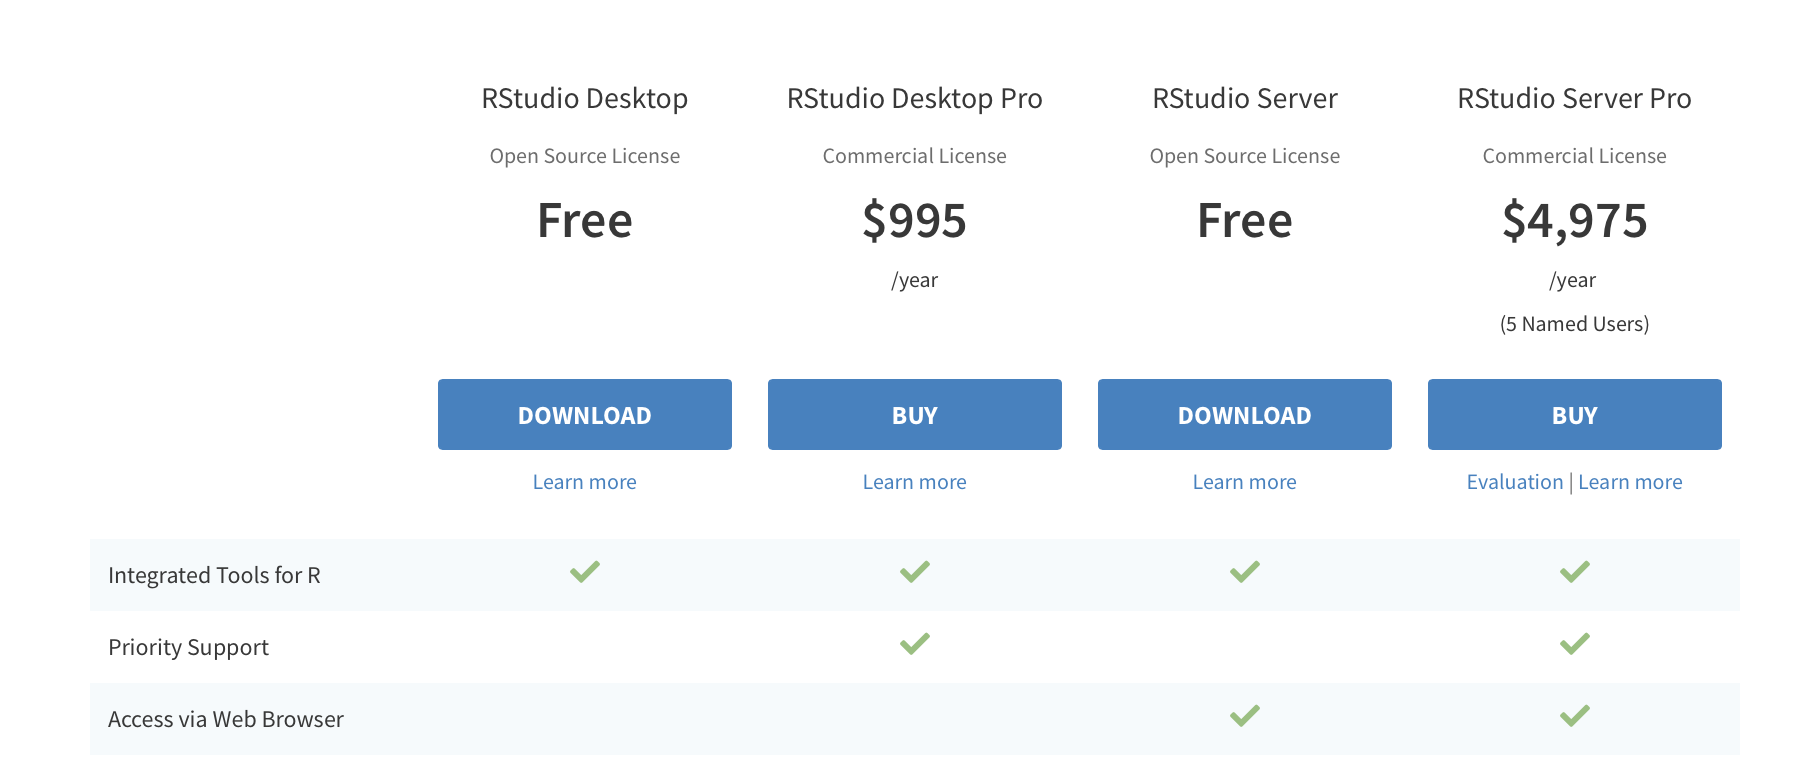
\includegraphics[width=0.8\linewidth]{/Users/lilymedina/Documents/GitHub/theory_and_practice_of_field_experiments/Book/Images/new_rstudio} \caption{Seleccione "Download" en la columna "RStudio Desktop Open Source License".}\label{fig:rstudiopng}
\end{figure}

\begin{figure}
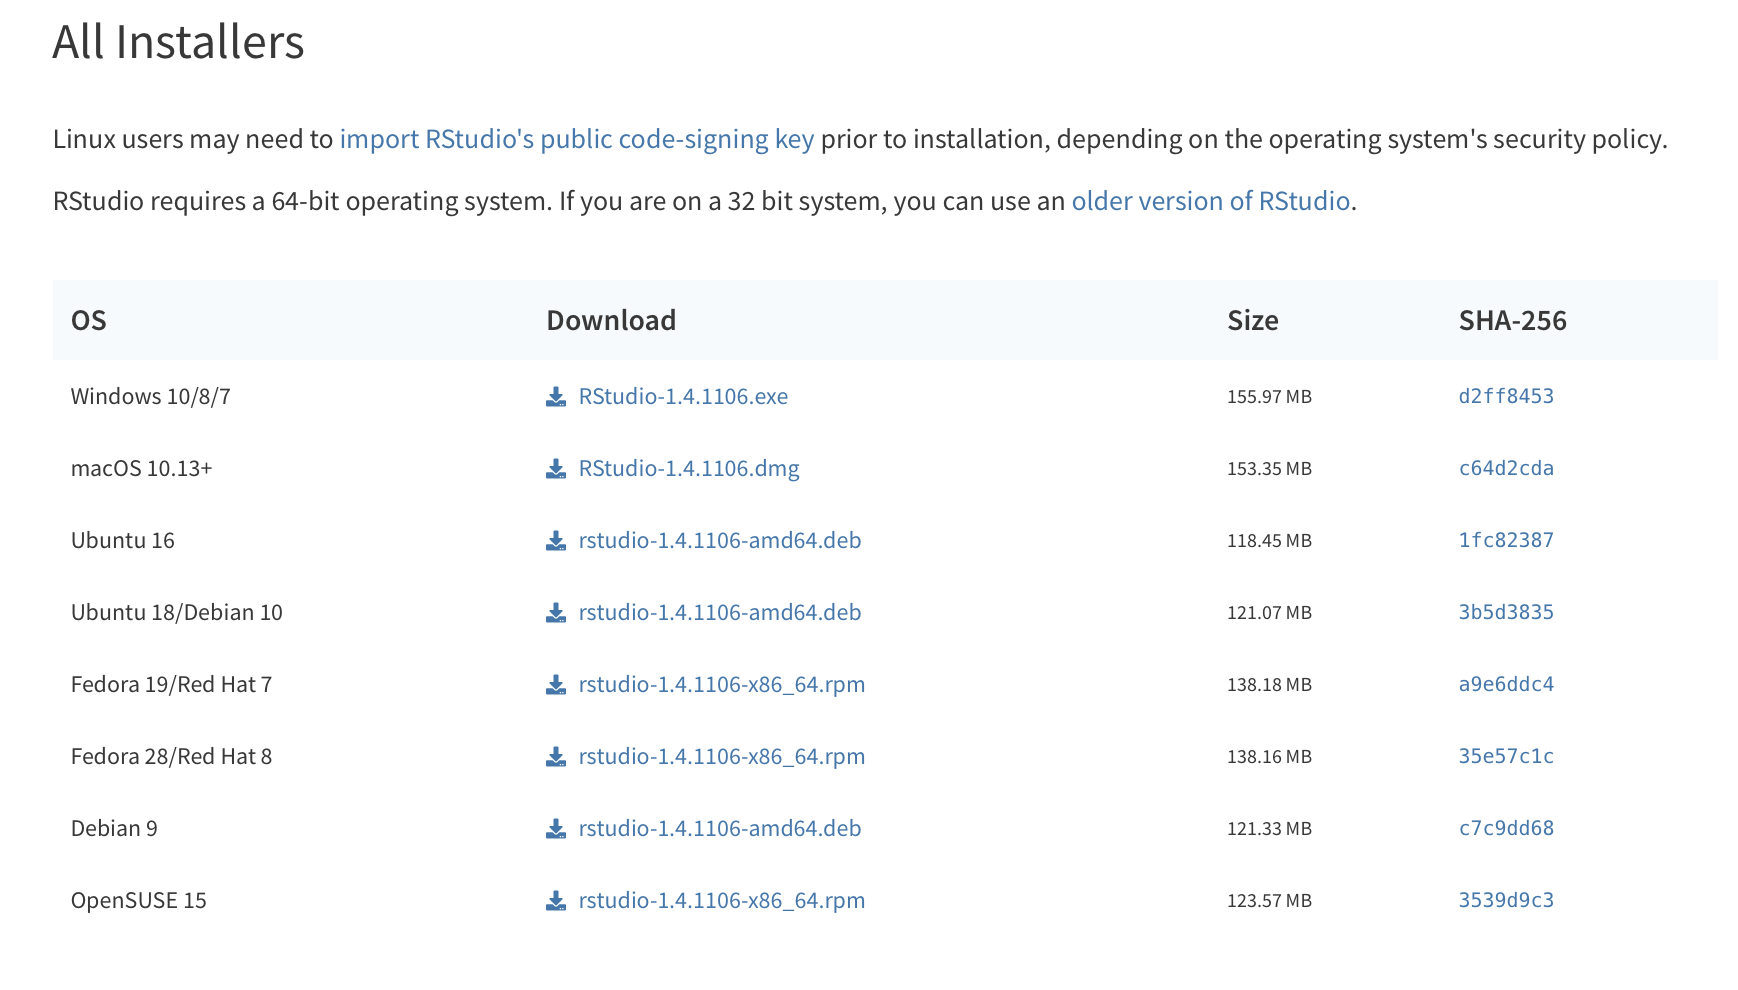
\includegraphics[width=0.8\linewidth]{Images/rstudio_download} \caption{Seleccione el link de Windows 10/8/7 para Windows o el link Mac OS X 10.13+ para Mac.}\label{fig:rstudiodownload}
\end{figure}

\hypertarget{interfaz-de-rstudio}{%
\section{Interfaz de RStudio}\label{interfaz-de-rstudio}}

Usted verá tres paneles la primera vez que ejecute RStudio, como se muestra en la Figura B.3 a continuación.

\begin{itemize}
\tightlist
\item
  Consola (panel izquierdo)
\item
  Entorno e Historial (panel superior derecho)
\item
  Misceláneo (panel inferior derecho)
\end{itemize}

\begin{figure}
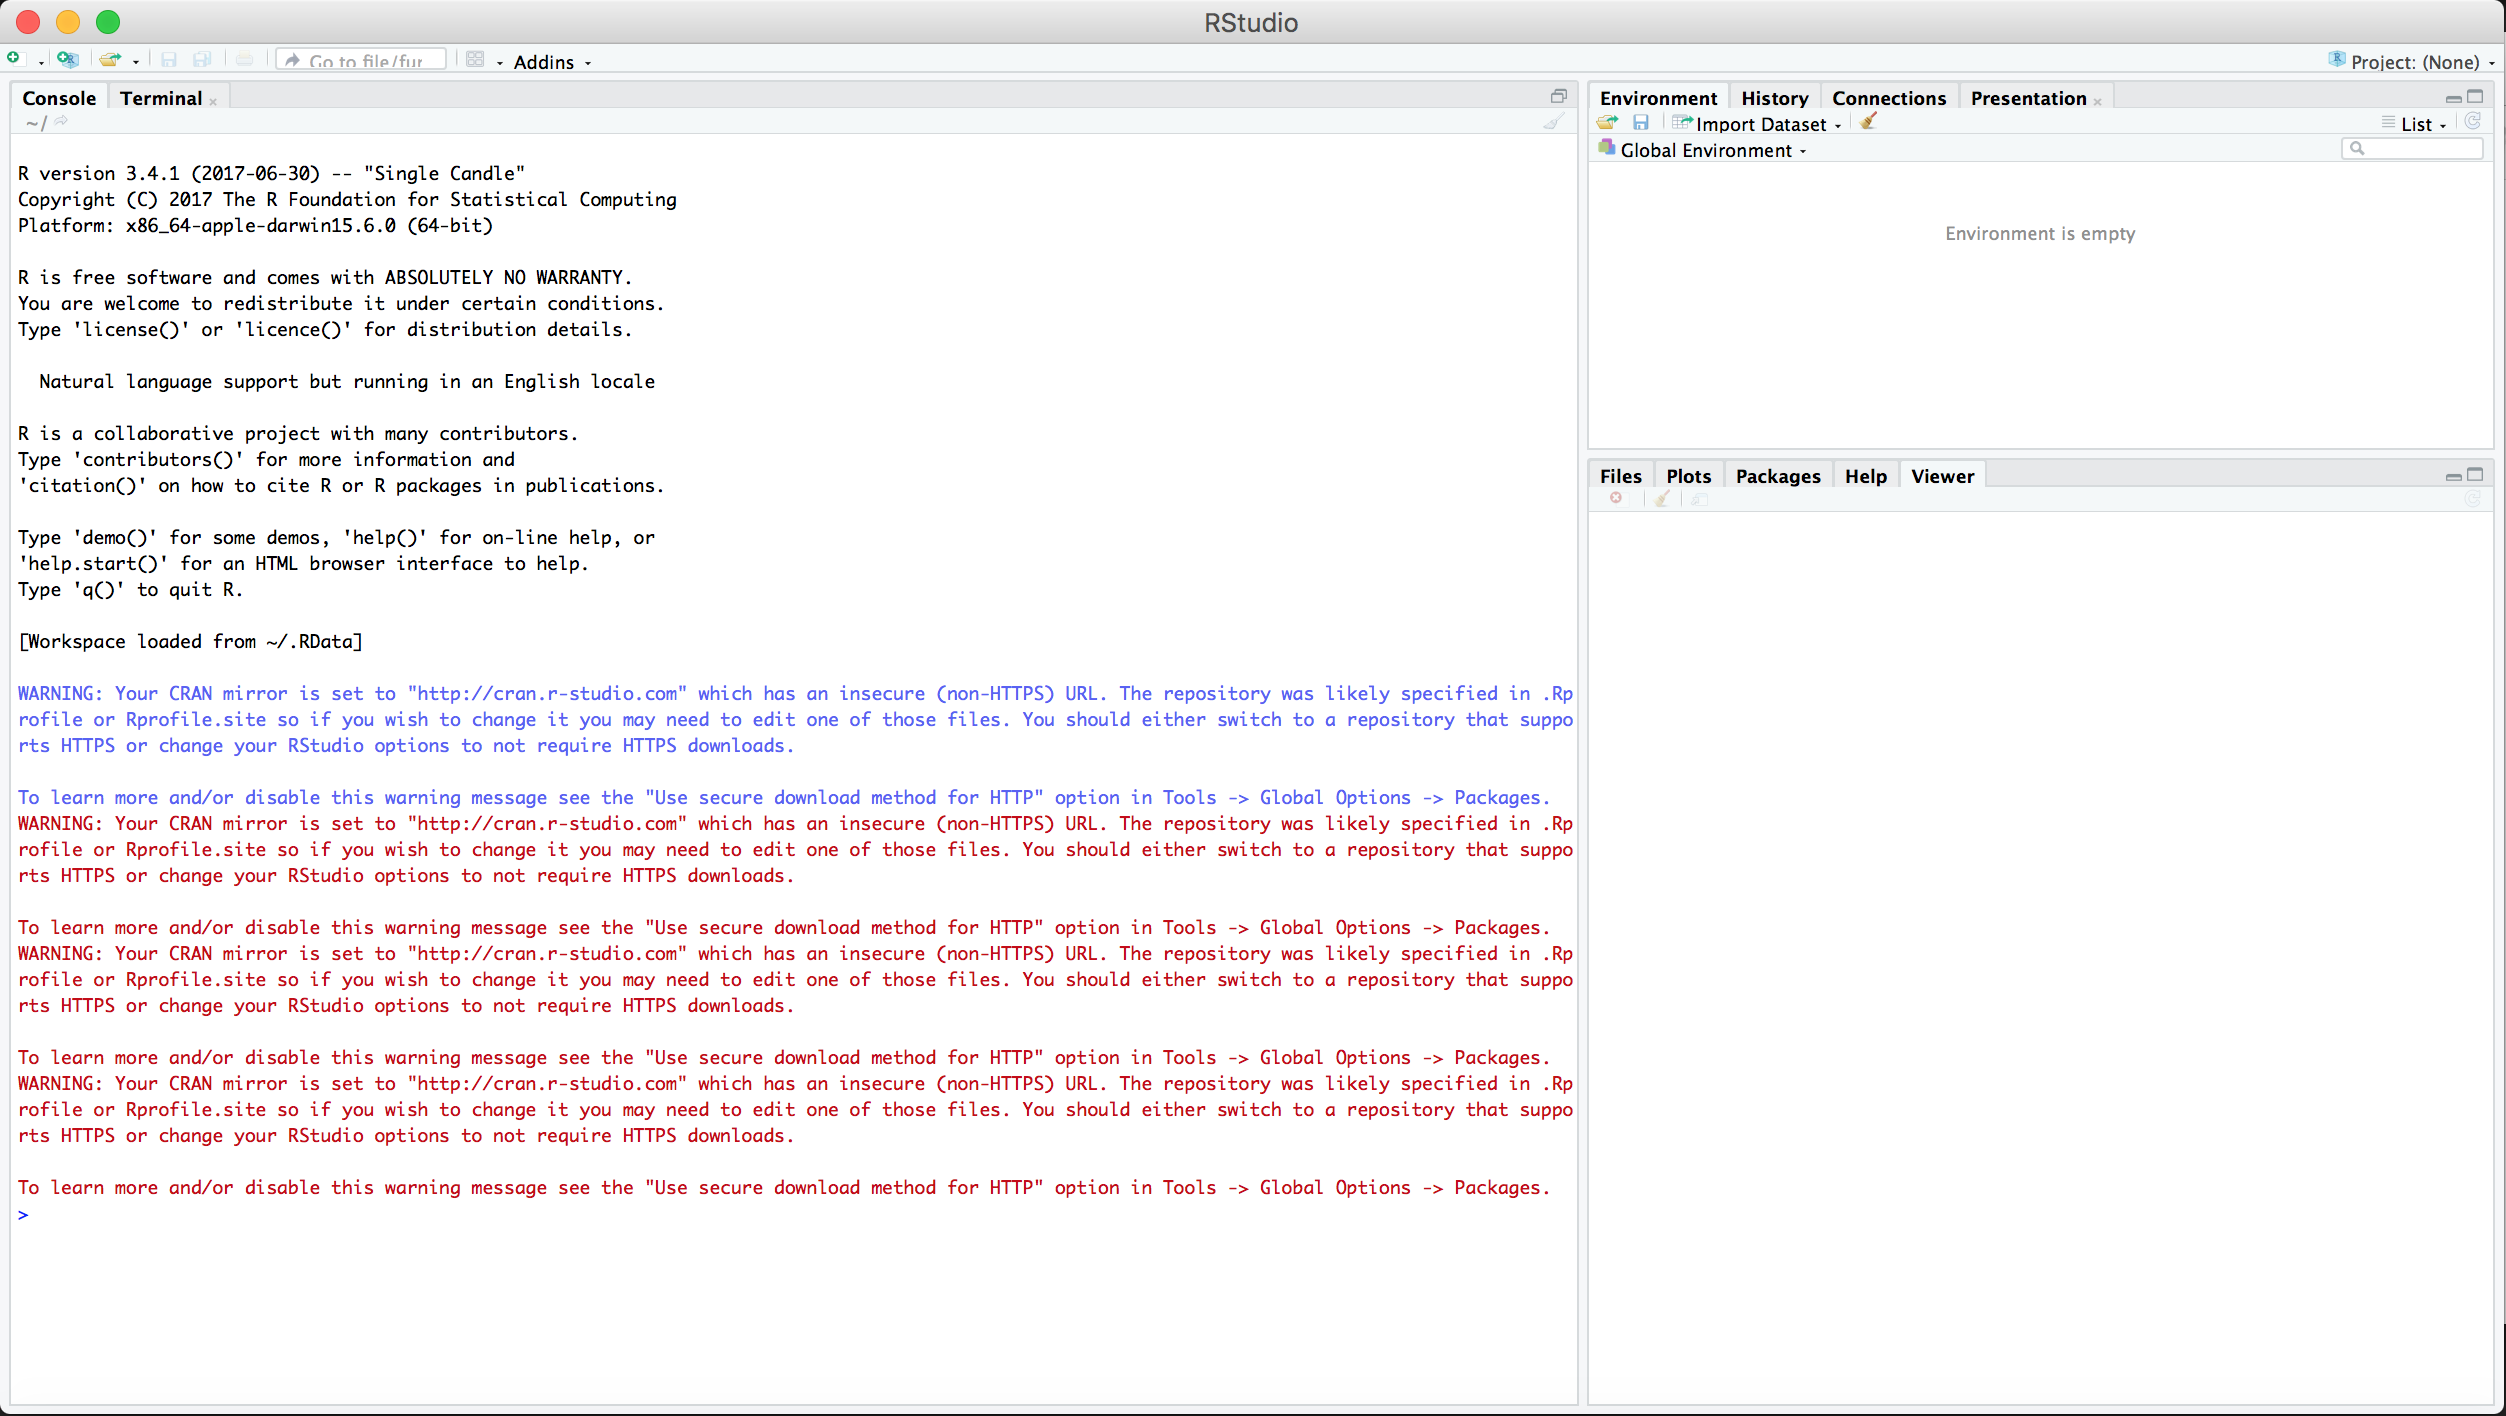
\includegraphics[width=0.8\linewidth]{Images/rstudio_intro} \caption{Cuando se abre RStudio, hay tres paneles visibles:  la Consola (panel izquierdo), Entorno e Historial (panel superior derecho) y  Misceláneo (panel inferior derecho).}\label{fig:rstudiointro}
\end{figure}

\hypertarget{consola}{%
\subsection{Consola}\label{consola}}

Puede ejecutar todas las operaciones directamente en la consola. Por ejemplo, si ingresa \texttt{4\ +\ 4} y presiona la tecla Enter/Return, la consola devolverá \texttt{{[}1{]}\ 8}.

Para asegurarnos que todos estén preparados para usar R en los Learning Days, les pedimos a los participantes que ejecuten una línea de código en particular en la consola para descargar varios paquetes de R. Los paquetes son fragmentos de código reproducible que permiten un análisis más eficiente en R. Para ejecutar estas líneas, copie el siguiente código en la Consola y presione la tecla ``Enter''/``Intro''. Tenga en cuenta que se requiere conexión a internet para poder descargar paquetes.

\begin{Shaded}
\begin{Highlighting}[]
\FunctionTok{install.packages}\NormalTok{(}\FunctionTok{c}\NormalTok{(}
  \StringTok{"ggplot2"}\NormalTok{, }\StringTok{"dplyr"}\NormalTok{, }\StringTok{"AER"}\NormalTok{, }\StringTok{"arm"}\NormalTok{, }\StringTok{"MASS"}\NormalTok{, }\StringTok{"sandwich"}\NormalTok{,}
  \StringTok{"lmtest"}\NormalTok{, }\StringTok{"estimatr"}\NormalTok{, }\StringTok{"coin"}\NormalTok{, }\StringTok{"randomizr"}\NormalTok{, }\StringTok{"DeclareDesign"}
\NormalTok{))}
\end{Highlighting}
\end{Shaded}

Si los paquetes son descargados correctamente, su consola se deberá ver como la figura B.4, excepto que las URL variarán de acuerdo a su ubicación.

\begin{figure}
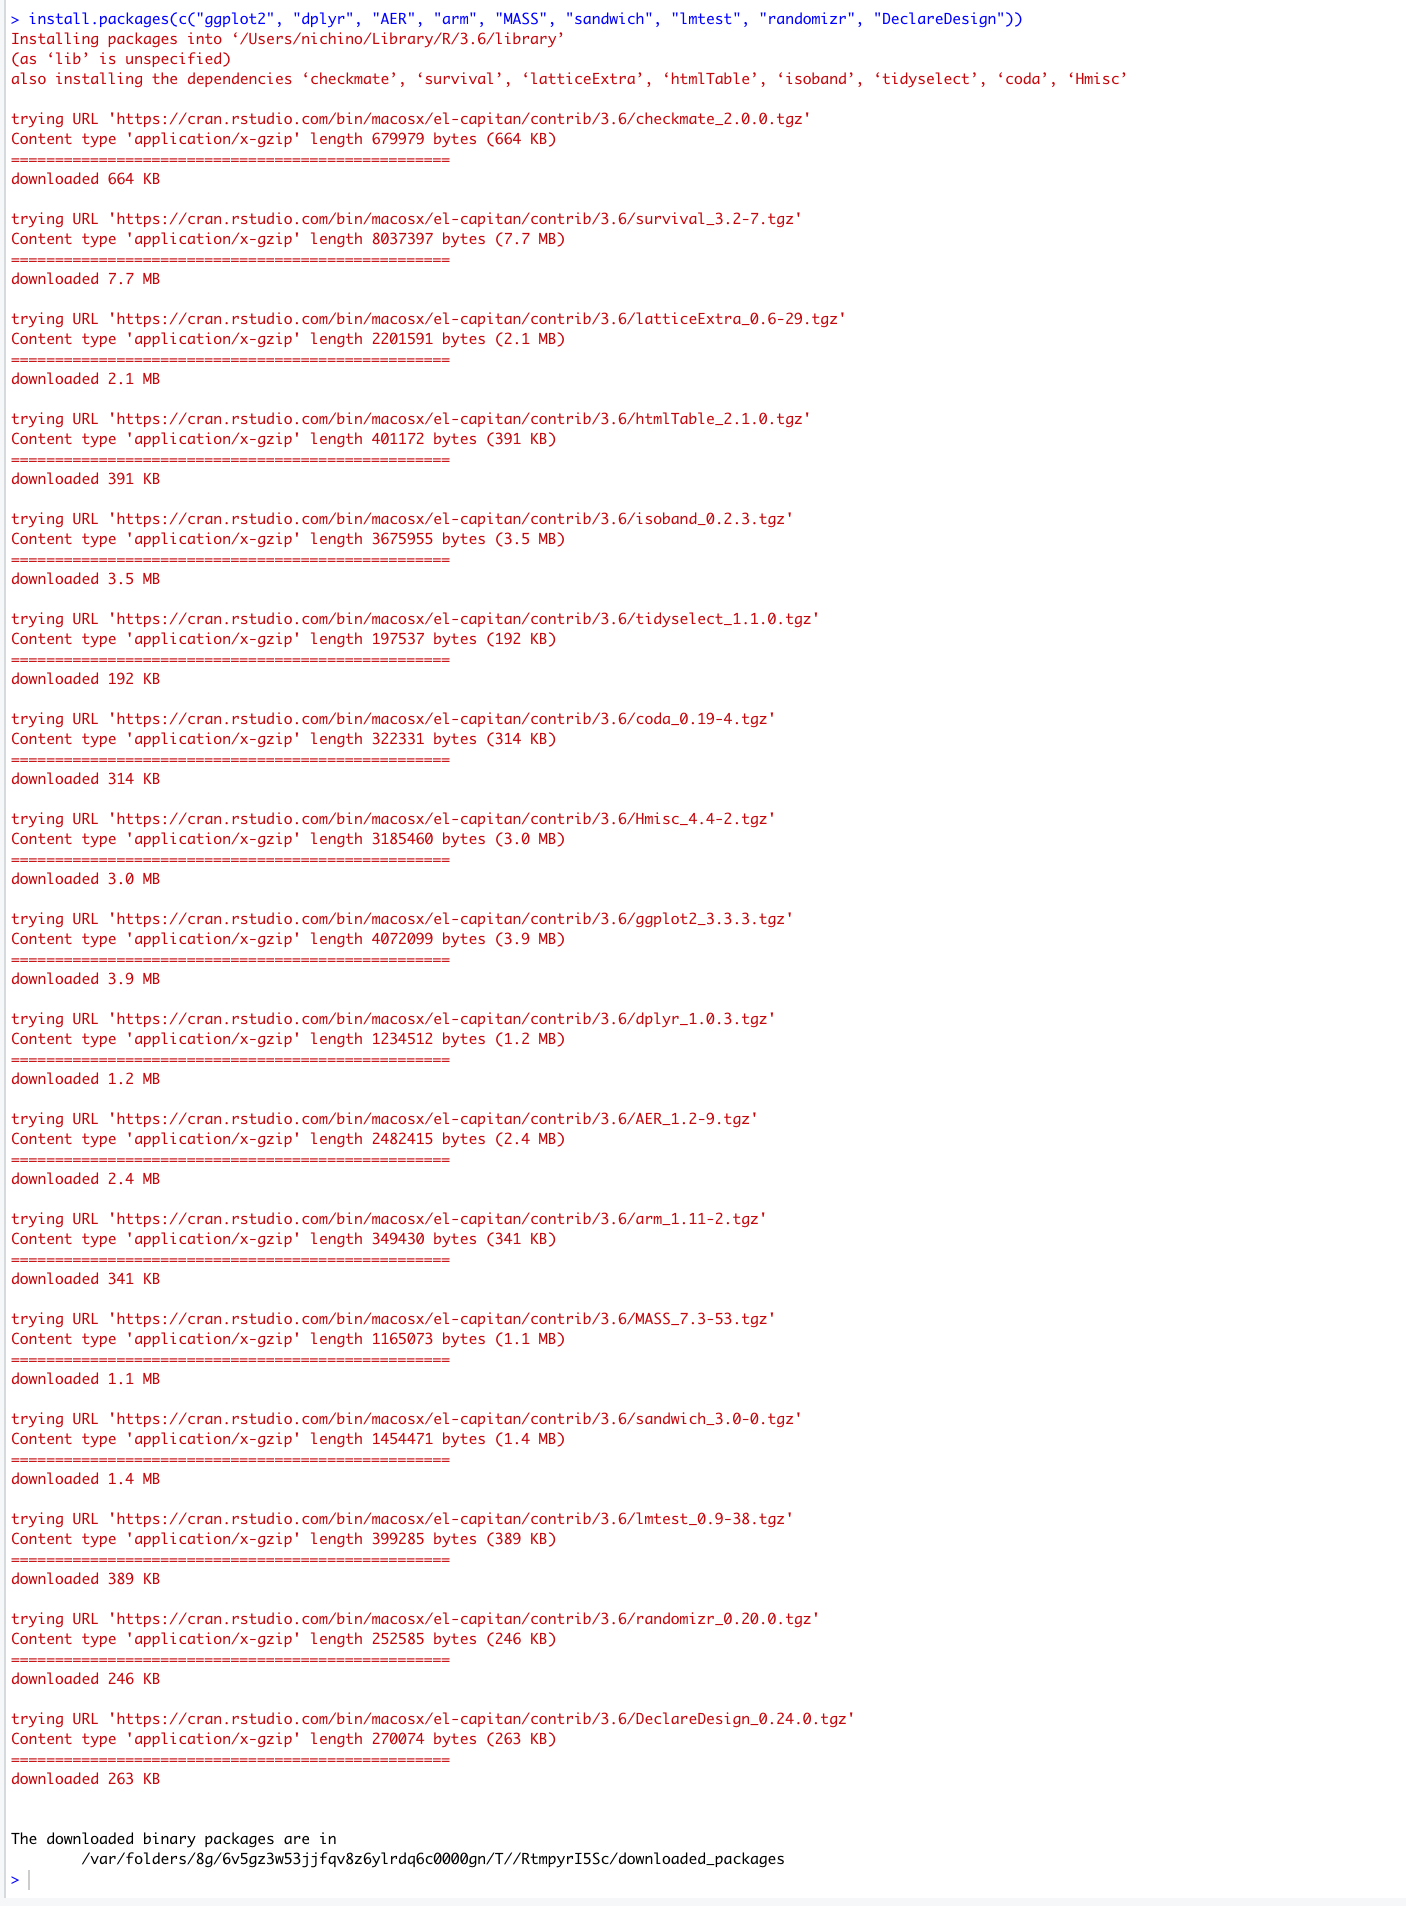
\includegraphics[width=0.4\linewidth]{Images/console2a} \caption{Un imagen de la Consola después de ejecutrar las tres lineas de códico indicadas arriba.}\label{fig:console2}
\end{figure}

\hypertarget{editor}{%
\subsection{Editor}\label{editor}}

Para escribir y guardar código reproducible se utiliza un cuarto panel, el Editor. Para abrir el Editor, haga clic en el icono con una página en blanco con un signo más en la esquina superior izquierda de la interfaz de RStudio y seleccione \texttt{R\ Script}, tal como se ve en la Figura B.5.

\begin{figure}
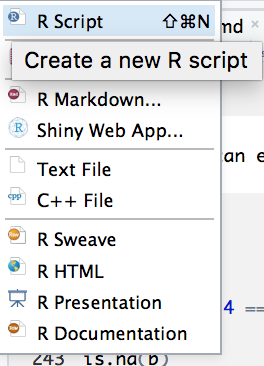
\includegraphics[width=0.6\linewidth]{Images/new_script} \caption{Para crear un nuevo archivo de R y abrir el Editor seleccione `R Script` del menú que se despliega.}\label{fig:newscript}
\end{figure}

Una vez que se abre un nuevo archivo de R (R script), debe haber cuatro paneles en la interfaz de RStudio, incluyendo el panel del Editor. Podemos ejecutar aritmética simple ingresando una fórmula en el Editor y presionando \texttt{Control\ +\ Enter} (Windows) o \texttt{Command\ +\ Enter} (Mac). La fórmula y la ``respuesta'' aparecerán en la Consola, tal como se muestra en la Figura B.6. Las casillas rojas son agregadas para enfatizar.

\begin{figure}
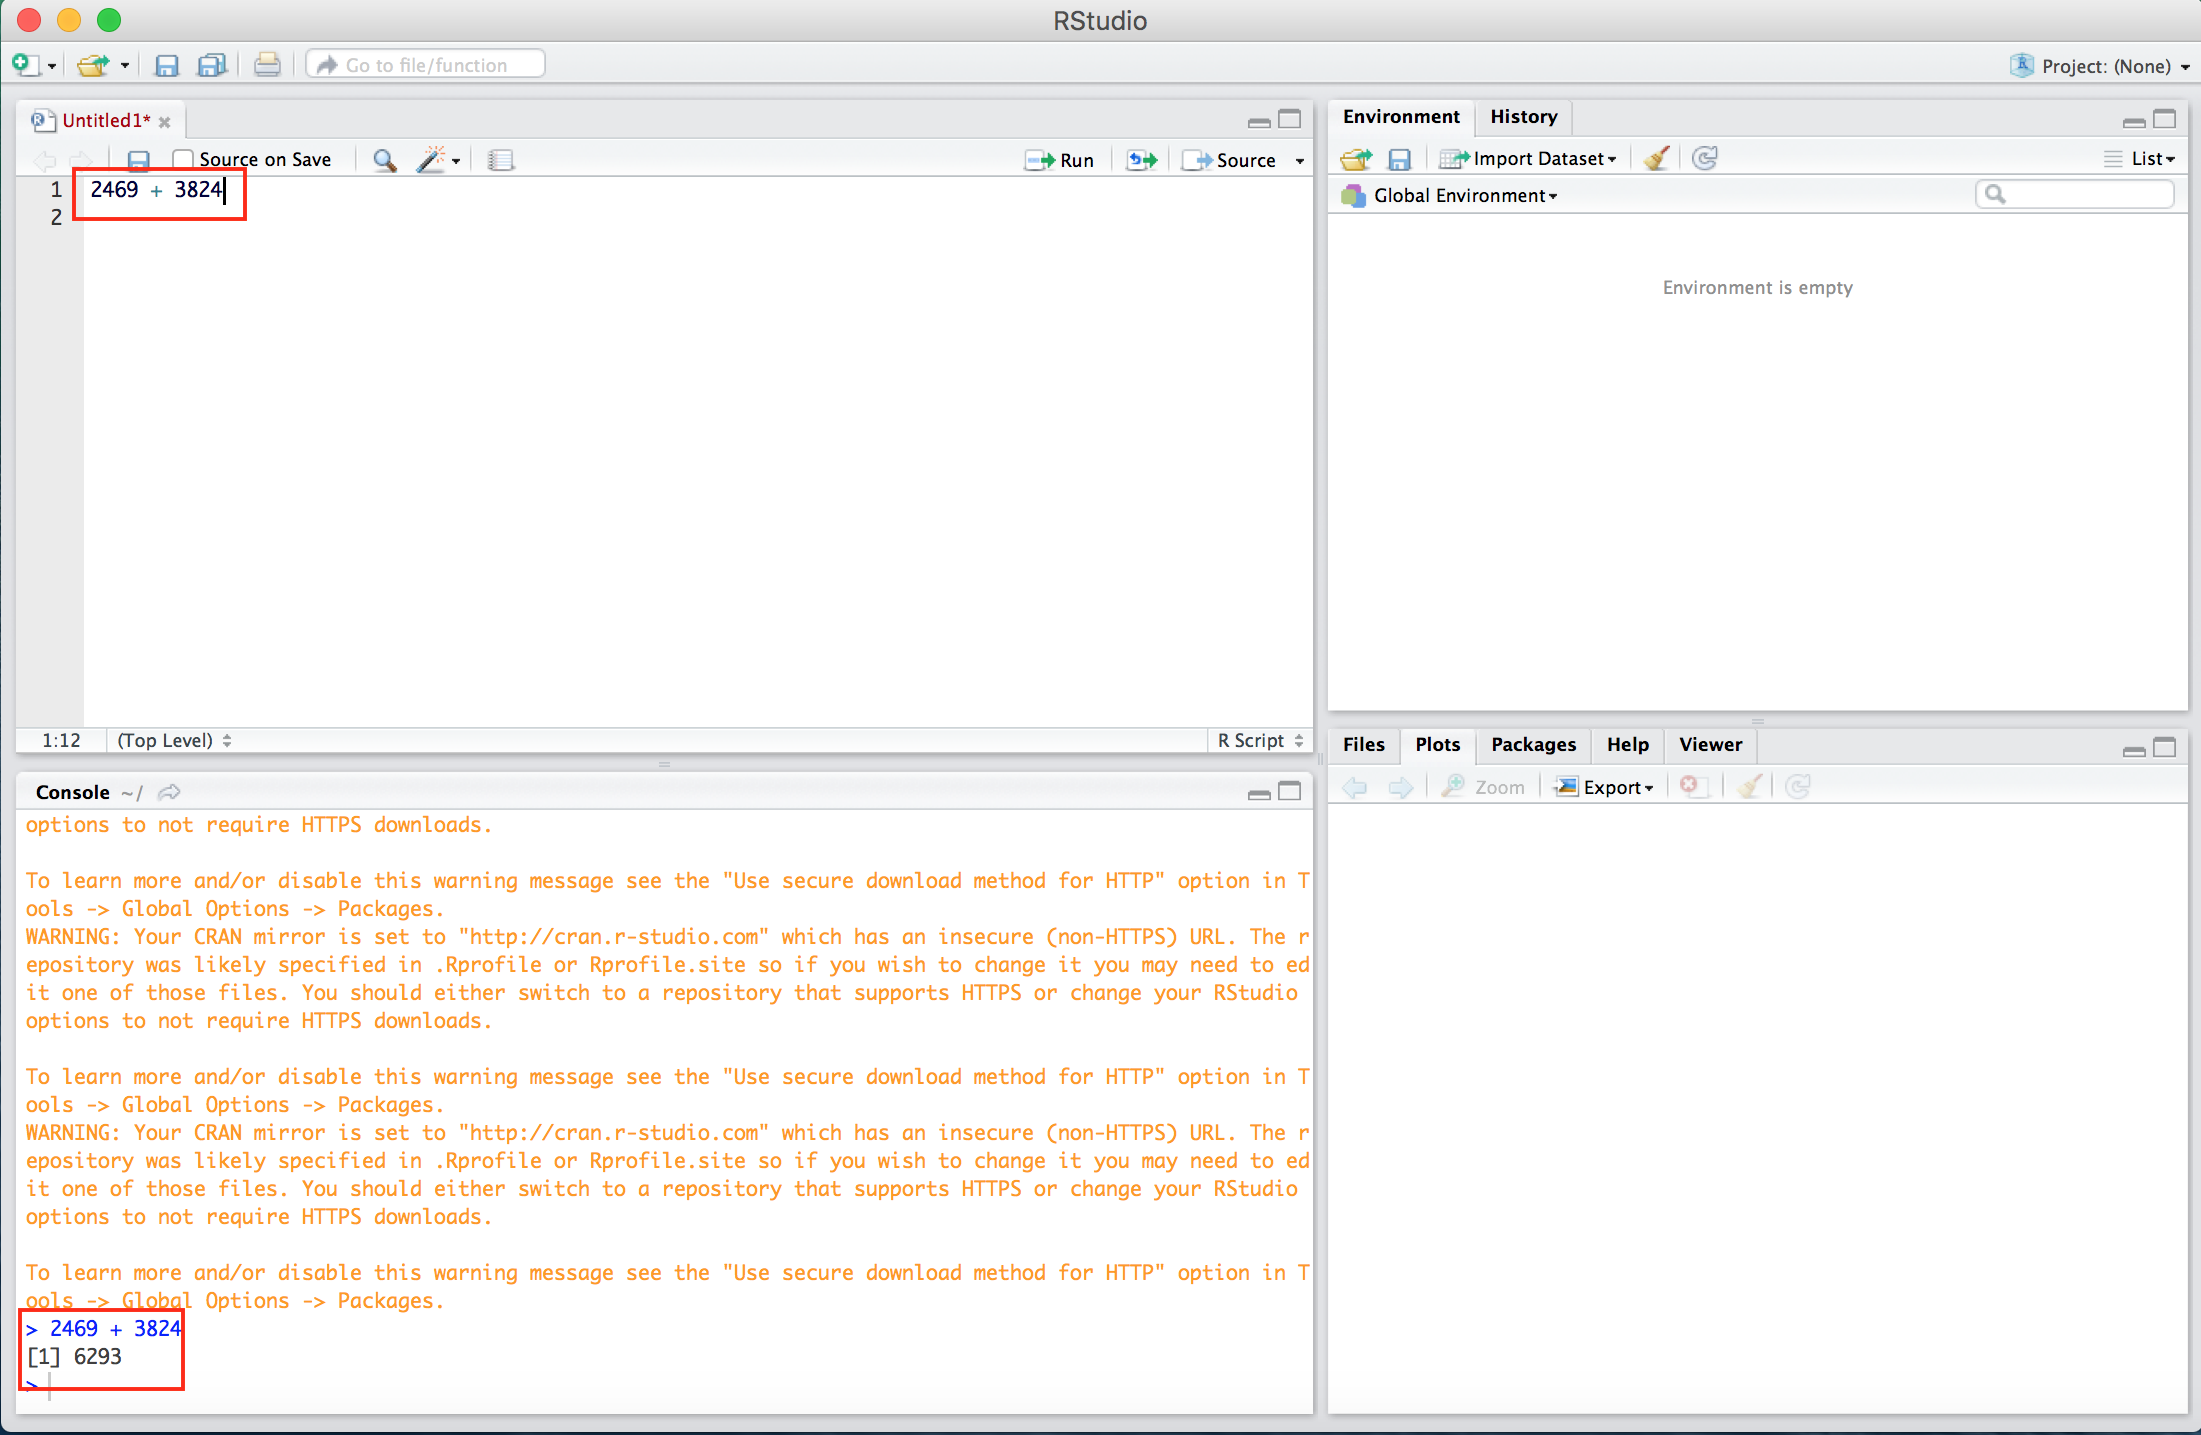
\includegraphics[width=0.6\linewidth]{Images/first_addition} \caption{Una expresióna aritmética se escribe en el Editor y se evalua en la Consola. Los recuadros rojos son para dar énfasis.}\label{fig:firstaddition}
\end{figure}

R se puede utilizar para cualquier operación aritmética, incluidas, entre otras, la suma (\texttt{+}), la resta (\texttt{-}), la multiplicación escalar (\texttt{*}), la división (\texttt{/}) y la exponenciación (\texttt{\^{}} ).

\hypertarget{entorno-historial-y-otros}{%
\subsection{Entorno, historial y otros}\label{entorno-historial-y-otros}}

Más allá de las funciones básicas también podemos almacenar valores, datos y funciones en el entorno global. Para asignar un valor a una variable, use el operador \texttt{\textless{}-}. Todos los valores, funciones y datos almacenados aparecerán en la pestaña Entorno del panel superior derecho. En la Figura B.7, definimos la variable \texttt{t} para tomar el valor \(3 \times \frac {6}{14}\). Como podemos ver \texttt{t} está almacenada en \emph{Values}.

También cargamos un conjunto de datos. Aquí, ``ChickWeight'' es un conjunto de datos integrado en R. La mayoría de los conjuntos de datos se cargarán desde la web u otros archivos en su computadora a través de un método alternativo. Podemos ver que ChickWeight contiene 578 observaciones de 4 variables y se almacena en el entorno. Al hacer clic en el nombre ChickWeight, ingresará una pestaña con el conjunto de datos en la ventana del Editor.

\begin{figure}
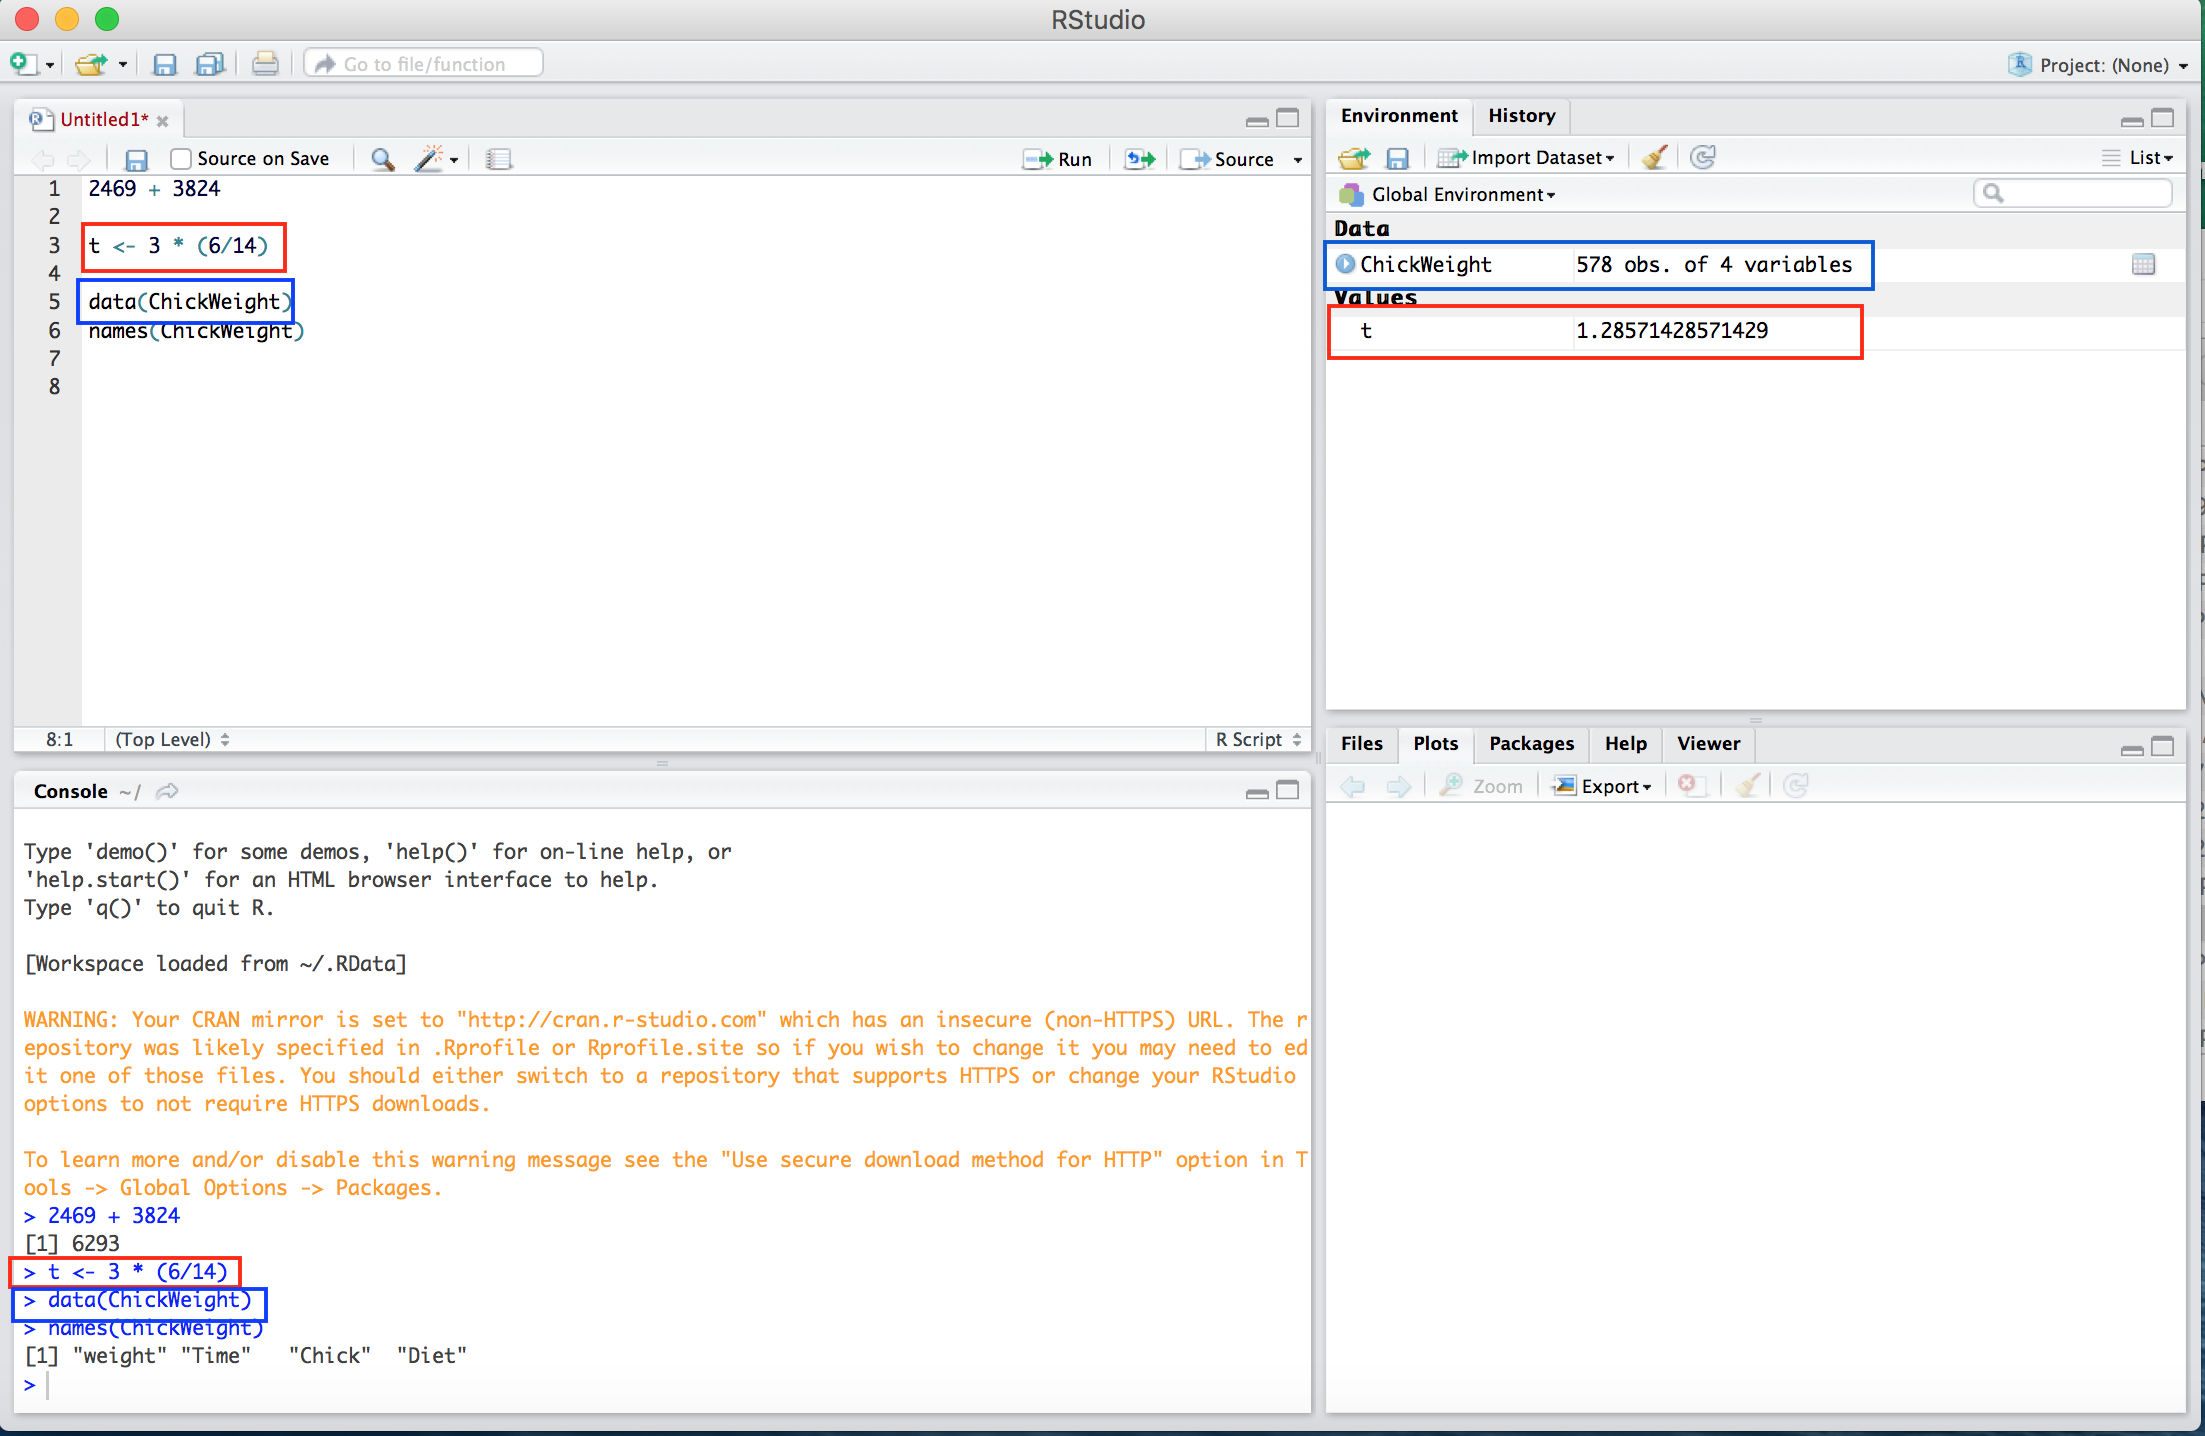
\includegraphics[width=0.6\linewidth]{Images/save_data} \caption{El valor 3 * (6/14) es asignado a la variable t (en rojo) y el conjunto de datos ChickWeight se guarda en el Entorno (en azul). Los recudros son para dar énfasis.}\label{fig:savedata}
\end{figure}

Los talleres de los Learning Days utilizan muchas herramientas en R para analizar y explorar datos. Por ahora, podemos aprender algunas herramientas básicas para examinar los datos. La función \texttt{head()} nos permite ver las primeras seis filas del conjunto de datos. \texttt{summary()} resume cada una de las columnas del conjunto de datos y \texttt{dim()} proporciona las dimensiones del conjunto de datos, primero el número de filas y luego las columnas.

\begin{Shaded}
\begin{Highlighting}[]
\FunctionTok{head}\NormalTok{(ChickWeight) }\CommentTok{\# Primeras 6 observaciones de los datos}
\end{Highlighting}
\end{Shaded}

\begin{verbatim}
  weight Time Chick Diet
1     42    0     1    1
2     51    2     1    1
3     59    4     1    1
4     64    6     1    1
5     76    8     1    1
6     93   10     1    1
\end{verbatim}

\begin{Shaded}
\begin{Highlighting}[]
\FunctionTok{summary}\NormalTok{(ChickWeight) }\CommentTok{\# Resumen de todas las variables}
\end{Highlighting}
\end{Shaded}

\begin{verbatim}
     weight         Time          Chick     Diet   
 Min.   : 35   Min.   : 0.0   13     : 12   1:220  
 1st Qu.: 63   1st Qu.: 4.0   9      : 12   2:120  
 Median :103   Median :10.0   20     : 12   3:120  
 Mean   :122   Mean   :10.7   10     : 12   4:118  
 3rd Qu.:164   3rd Qu.:16.0   17     : 12          
 Max.   :373   Max.   :21.0   19     : 12          
                              (Other):506          
\end{verbatim}

\begin{Shaded}
\begin{Highlighting}[]
\FunctionTok{dim}\NormalTok{(ChickWeight) }\CommentTok{\# Dimensiones de los datos; primero filas luego columnas}
\end{Highlighting}
\end{Shaded}

\begin{verbatim}
[1] 578   4
\end{verbatim}

A diferencia de cualquier otro software estadístico, R permite a los usuarios almacenar múltiples conjuntos de datos de diferentes dimensiones simultáneamente. Esta característica hace que R sea bastante flexible para el análisis de datos utilizando distintos métodos.

\hypertarget{misceluxe1neo}{%
\subsection{Misceláneo}\label{misceluxe1neo}}

R proporciona un conjunto de herramientas, que van desde funciones integradas para graficar (\texttt{plot}) hasta paquetes externos para estimaciones, modelos, gráfico de datos, etc. El último panel, Misceláneo, permite la visualización rápida de gráficos en RStudio. La Figura B.8 muestra cómo se ve una gráfica en este panel. En los Learning Days se explicara más en detalle cómo graficar datos. Por ahora no se preocupe por el código para graficar que aparece en el Editor.

\begin{figure}
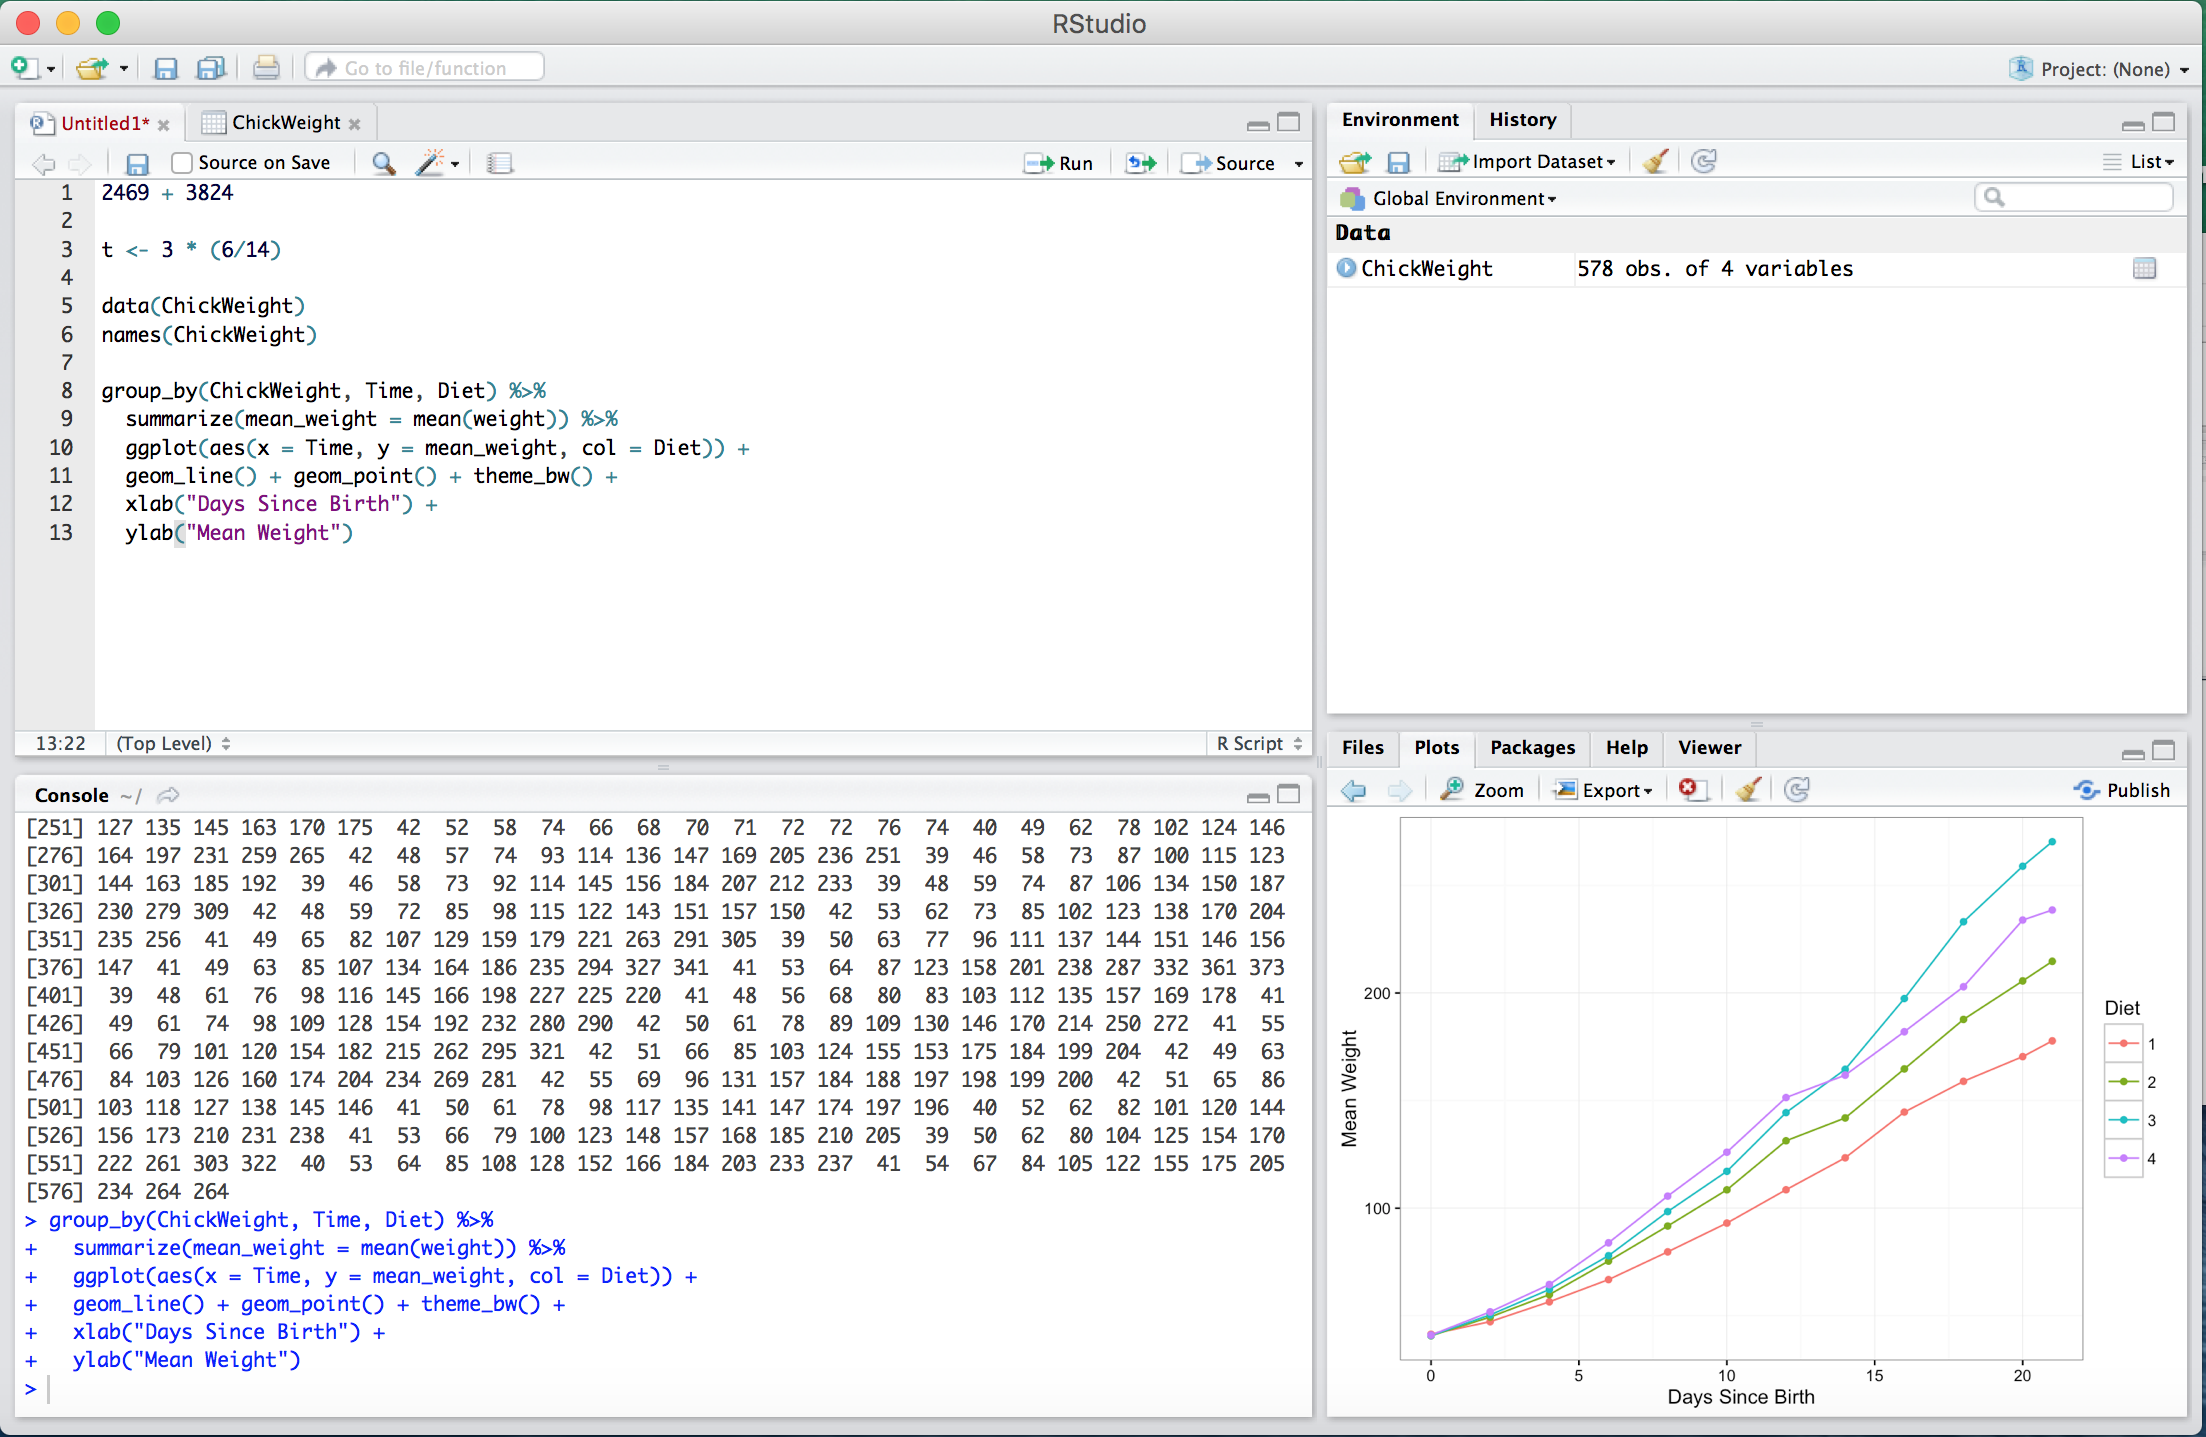
\includegraphics[width=0.6\linewidth]{Images/graph} \caption{Un ejemplo de una gráfica de datos hecha en R utilizando el conjunto de datos `ChickWeight`.}\label{fig:graph}
\end{figure}

\hypertarget{aprendiendo-a-usar-r}{%
\section{Aprendiendo a usar R}\label{aprendiendo-a-usar-r}}

\hypertarget{recursos-en-luxednea}{%
\subsection{Recursos en línea}\label{recursos-en-luxednea}}

Hay muchos recursos útiles en línea que lo ayudarán a familiarizarse con R. Nosotros recomendamos dos fuentes:

\begin{itemize}
\tightlist
\item
  Code School, que se ejecuta completamente a través de su navegador \url{https://www.codeschool.com/courses/try-r}.
\item
  Coursera, a través de un curso de programación R en línea organizado por la Universidad Johns Hopkins:

  \begin{enumerate}
  \def\labelenumi{\roman{enumi}.}
  \tightlist
  \item
    Vaya a {[}\url{https://www.coursera.org}{]} (\url{https://www.coursera.org})
  \item
    Cree una cuenta (¡es gratis!)
  \item
    Regístrese en R Programming en la Universidad de Johns Hopkins (instructor: Roger Peng) en la pestaña ``Courses''.
  \item
    Lea los materiales y vea los videos de la primera semana. Los videos de la primera semana duran aproximadamente 2.5 horas en total.
  \end{enumerate}
\end{itemize}

\hypertarget{pruxe1ctica-buxe1sica}{%
\subsection{Práctica básica}\label{pruxe1ctica-buxe1sica}}

Aquí proporcionamos algunos fragmentos de código para que se familiarice con algunas prácticas básicas en R. Le recomendamos que practique escribiendo los fragmentos de código en su Editor y luego revisando los resultados.

\hypertarget{configuraciuxf3n-de-una-sesiuxf3n-r}{%
\subsubsection{Configuración de una sesión R}\label{configuraciuxf3n-de-una-sesiuxf3n-r}}

En general, leemos otros archivos tales como datos o funciones en R y generamos resultados en forma de gráficos o tablas guardados en archivos que no están contenidos en una sesión de R. Para hacer esto, debemos darle a R una ``dirección'' en la que guardar dichos archivos. Puede ser más eficiente hacer esto configurando un directorio de trabajo, esto es, una ruta de archivo en la que se almacenan los archivos relevantes. Podemos identificar el directorio de trabajo actual usando \texttt{getwd()} y establecer uno nuevo usando \texttt{setwd()}. Tenga en cuenta que la sintaxis de estas rutas de archivo varía según el sistema operativo.

\begin{Shaded}
\begin{Highlighting}[]
\FunctionTok{getwd}\NormalTok{()}
\end{Highlighting}
\end{Shaded}

\begin{Shaded}
\begin{Highlighting}[]
\FunctionTok{setwd}\NormalTok{(}\StringTok{"\textasciitilde{}TaraLyn/EGAP Learning Days Admin/Workshop 2018\_2 (Uruguay)/"}\NormalTok{)}
\end{Highlighting}
\end{Shaded}

Es posible que usted necesite instalar paquetes adicionales a los enumerados anteriormente para ejecutar ciertas funciones. Para instalar paquetes se utiliza la función \texttt{install.packages("\ ")}, escribiendo el nombre del paquete entre comillas. Solo hace falta instalar los paquetes una vez.

\begin{Shaded}
\begin{Highlighting}[]
\FunctionTok{install.packages}\NormalTok{(}\StringTok{"randomizr"}\NormalTok{)}
\end{Highlighting}
\end{Shaded}

Una vez que se instala un paquete se puede cargar y acceder a él usando \texttt{library()} donde el nombre del paquete se inserta entre paréntesis (sin comillas "").

\begin{Shaded}
\begin{Highlighting}[]
\FunctionTok{library}\NormalTok{(randomizr)}
\end{Highlighting}
\end{Shaded}

Para borrar la memoria de R de los datos, funciones o valores almacenados que aparecen en la pestaña del entorno (Environment), use \texttt{rm(list\ =\ ls())}. Puede ser útil establecer una semilla de un número aleatorio para garantizar que sea posible replicar nuestro código en una sesión de R diferente. Esto es especialmente importante cuando trabajamos con métodos basados en simulación.

\begin{Shaded}
\begin{Highlighting}[]
\FunctionTok{rm}\NormalTok{(}\AttributeTok{list =} \FunctionTok{ls}\NormalTok{())}
\FunctionTok{set.seed}\NormalTok{(}\DecValTok{2018}\NormalTok{) }\CommentTok{\# Opcional: definir semilla para resultados replicables}
\end{Highlighting}
\end{Shaded}

\hypertarget{comandos-buxe1sicos-de-r}{%
\subsubsection{Comandos básicos de R}\label{comandos-buxe1sicos-de-r}}

A continuación, exploraremos algunos de los comandos básicos de R. Por ejemplo, para asignar un escalar (un elemento simple) a una variable, usamos el comando \texttt{\textless{}-} como mencionamos anteriormente:

\begin{Shaded}
\begin{Highlighting}[]
\CommentTok{\# "\textless{}{-}"  es el comando para asignar; Se utiliza para definir variables.}
\CommentTok{\# Por ejemplo:}
\NormalTok{(a }\OtherTok{\textless{}{-}} \DecValTok{5}\NormalTok{)}
\end{Highlighting}
\end{Shaded}

\begin{verbatim}
[1] 5
\end{verbatim}

También es posible que queramos asignar un vector de elementos a una variable. Aquí usamos el mismo comando \texttt{\textless{}-}, pero nos enfocamos en cómo crear el vector.

\begin{Shaded}
\begin{Highlighting}[]
\NormalTok{(b }\OtherTok{\textless{}{-}} \DecValTok{1}\SpecialCharTok{:}\DecValTok{10}\NormalTok{) }\CommentTok{\# ":"  se utiliza para crear una cadena de números enteros}
\end{Highlighting}
\end{Shaded}

\begin{verbatim}
 [1]  1  2  3  4  5  6  7  8  9 10
\end{verbatim}

\begin{Shaded}
\begin{Highlighting}[]
\NormalTok{(v }\OtherTok{\textless{}{-}} \FunctionTok{c}\NormalTok{(}\DecValTok{1}\NormalTok{, }\DecValTok{3}\NormalTok{, }\DecValTok{2}\NormalTok{, }\DecValTok{4}\NormalTok{, pi)) }\CommentTok{\#  c() se utiliza para crear un vector}
\end{Highlighting}
\end{Shaded}

\begin{verbatim}
[1] 1.000 3.000 2.000 4.000 3.142
\end{verbatim}

\begin{Shaded}
\begin{Highlighting}[]
\CommentTok{\#   cuyos elementos pueden ser de cualquier tipo}
\end{Highlighting}
\end{Shaded}

Podemos referirnos a los elementos de un vector indicando su posición en el vector entre corchetes \texttt{{[}{]}}.

\begin{Shaded}
\begin{Highlighting}[]
\CommentTok{\# Consultar los elementos de un vector:}
\NormalTok{b[}\DecValTok{1}\NormalTok{] }\CommentTok{\# Devuelve la 1ra posición del vector}
\end{Highlighting}
\end{Shaded}

\begin{verbatim}
[1] 1
\end{verbatim}

\begin{Shaded}
\begin{Highlighting}[]
\NormalTok{b[}\DecValTok{5}\SpecialCharTok{:}\DecValTok{4}\NormalTok{] }\CommentTok{\# Devuelve las posiciones 5 y 4; en ese orden}
\end{Highlighting}
\end{Shaded}

\begin{verbatim}
[1] 5 4
\end{verbatim}

\begin{Shaded}
\begin{Highlighting}[]
\NormalTok{b[}\SpecialCharTok{{-}}\DecValTok{1}\NormalTok{] }\CommentTok{\# Devuelve todas las posiciones menos la primera}
\end{Highlighting}
\end{Shaded}

\begin{verbatim}
[1]  2  3  4  5  6  7  8  9 10
\end{verbatim}

\begin{Shaded}
\begin{Highlighting}[]
\CommentTok{\# Devuelve todas las posiciones para las cuales se indica "TRUE"}
\NormalTok{b[}\FunctionTok{c}\NormalTok{(}\ConstantTok{TRUE}\NormalTok{, }\ConstantTok{FALSE}\NormalTok{, }\ConstantTok{TRUE}\NormalTok{, }\ConstantTok{FALSE}\NormalTok{, }\ConstantTok{FALSE}\NormalTok{, }\ConstantTok{TRUE}\NormalTok{, }\ConstantTok{TRUE}\NormalTok{, }\ConstantTok{FALSE}\NormalTok{, }\ConstantTok{FALSE}\NormalTok{, }\ConstantTok{FALSE}\NormalTok{)]}
\end{Highlighting}
\end{Shaded}

\begin{verbatim}
[1] 1 3 6 7
\end{verbatim}

\begin{Shaded}
\begin{Highlighting}[]
\CommentTok{\# Para asignar valores a posiciones específicas en un vector}
\NormalTok{b[}\DecValTok{5}\NormalTok{] }\OtherTok{\textless{}{-}} \DecValTok{0}
\end{Highlighting}
\end{Shaded}

Hay un conjunto de funciones integradas que se pueden aplicar a vectores como \texttt{b}.

\begin{Shaded}
\begin{Highlighting}[]
\FunctionTok{sum}\NormalTok{(b) }\CommentTok{\# Suma de todos los elementos}
\end{Highlighting}
\end{Shaded}

\begin{verbatim}
[1] 50
\end{verbatim}

\begin{Shaded}
\begin{Highlighting}[]
\FunctionTok{mean}\NormalTok{(b) }\CommentTok{\# Promedio de todos los elementos}
\end{Highlighting}
\end{Shaded}

\begin{verbatim}
[1] 5
\end{verbatim}

\begin{Shaded}
\begin{Highlighting}[]
\FunctionTok{max}\NormalTok{(b) }\CommentTok{\# Máximo de todos los elementos}
\end{Highlighting}
\end{Shaded}

\begin{verbatim}
[1] 10
\end{verbatim}

\begin{Shaded}
\begin{Highlighting}[]
\FunctionTok{min}\NormalTok{(b) }\CommentTok{\# Mínimo de todos los elementos}
\end{Highlighting}
\end{Shaded}

\begin{verbatim}
[1] 0
\end{verbatim}

\begin{Shaded}
\begin{Highlighting}[]
\FunctionTok{sd}\NormalTok{(b) }\CommentTok{\# Desviación estándar de todos los elementos}
\end{Highlighting}
\end{Shaded}

\begin{verbatim}
[1] 3.496
\end{verbatim}

\begin{Shaded}
\begin{Highlighting}[]
\FunctionTok{var}\NormalTok{(b) }\CommentTok{\# Varianza de todos los elementos}
\end{Highlighting}
\end{Shaded}

\begin{verbatim}
[1] 12.22
\end{verbatim}

También podemos aplicar transformaciones aritméticas a los elementos de un vector:

\begin{Shaded}
\begin{Highlighting}[]
\NormalTok{b}\SpecialCharTok{\^{}}\DecValTok{2} \CommentTok{\# Eleva c/u de los elementos al cuadrado}
\end{Highlighting}
\end{Shaded}

\begin{verbatim}
 [1]   1   4   9  16   0  36  49  64  81 100
\end{verbatim}

\begin{Shaded}
\begin{Highlighting}[]
\NormalTok{b}\SpecialCharTok{\^{}}\NormalTok{.}\DecValTok{5} \CommentTok{\# Calcula la raíz cuadrada de los elementos}
\end{Highlighting}
\end{Shaded}

\begin{verbatim}
 [1] 1.000 1.414 1.732 2.000 0.000 2.449 2.646 2.828 3.000 3.162
\end{verbatim}

\begin{Shaded}
\begin{Highlighting}[]
\FunctionTok{log}\NormalTok{(b) }\CommentTok{\# Calcula el logaritmo de los elementos}
\end{Highlighting}
\end{Shaded}

\begin{verbatim}
 [1] 0.0000 0.6931 1.0986 1.3863   -Inf 1.7918 1.9459 2.0794 2.1972 2.3026
\end{verbatim}

\begin{Shaded}
\begin{Highlighting}[]
\FunctionTok{exp}\NormalTok{(b)[}\DecValTok{1}\SpecialCharTok{:}\DecValTok{6}\NormalTok{] }\CommentTok{\# e elevado a la b. sólo mostramos las posiciones 1 a 6,}
\end{Highlighting}
\end{Shaded}

\begin{verbatim}
[1]   2.718   7.389  20.086  54.598   1.000 403.429
\end{verbatim}

\begin{Shaded}
\begin{Highlighting}[]
\CommentTok{\# por razones de diagramación pero la operación se  aplica a todo el vector b}
\end{Highlighting}
\end{Shaded}

Finalmente, podemos evaluar condiciones lógicas (es decir, ``¿es verdadera la condición X?'\,') En todos los elementos de un vector:

\begin{Shaded}
\begin{Highlighting}[]
\NormalTok{b }\SpecialCharTok{==} \DecValTok{2} \CommentTok{\# Es igual a ?}
\end{Highlighting}
\end{Shaded}

\begin{verbatim}
 [1] FALSE  TRUE FALSE FALSE FALSE FALSE FALSE FALSE FALSE FALSE
\end{verbatim}

\begin{Shaded}
\begin{Highlighting}[]
\NormalTok{b }\SpecialCharTok{\textless{}} \DecValTok{5} \CommentTok{\# Es menor que}
\end{Highlighting}
\end{Shaded}

\begin{verbatim}
 [1]  TRUE  TRUE  TRUE  TRUE  TRUE FALSE FALSE FALSE FALSE FALSE
\end{verbatim}

\begin{Shaded}
\begin{Highlighting}[]
\NormalTok{b }\SpecialCharTok{\textgreater{}=} \DecValTok{5} \CommentTok{\# Es mayor o igual que}
\end{Highlighting}
\end{Shaded}

\begin{verbatim}
 [1] FALSE FALSE FALSE FALSE FALSE  TRUE  TRUE  TRUE  TRUE  TRUE
\end{verbatim}

\begin{Shaded}
\begin{Highlighting}[]
\NormalTok{b }\SpecialCharTok{\textless{}=} \DecValTok{5} \SpecialCharTok{|}\NormalTok{ b }\SpecialCharTok{/} \DecValTok{4} \SpecialCharTok{==} \DecValTok{2} \CommentTok{\# | signfica "o"}
\end{Highlighting}
\end{Shaded}

\begin{verbatim}
 [1]  TRUE  TRUE  TRUE  TRUE  TRUE FALSE FALSE  TRUE FALSE FALSE
\end{verbatim}

\begin{Shaded}
\begin{Highlighting}[]
\NormalTok{b }\SpecialCharTok{\textgreater{}} \DecValTok{2} \SpecialCharTok{\&}\NormalTok{ b }\SpecialCharTok{\textless{}} \DecValTok{9} \CommentTok{\# \& significa "y"}
\end{Highlighting}
\end{Shaded}

\begin{verbatim}
 [1] FALSE FALSE  TRUE  TRUE FALSE  TRUE  TRUE  TRUE FALSE FALSE
\end{verbatim}

\begin{Shaded}
\begin{Highlighting}[]
\FunctionTok{is.na}\NormalTok{(b) }\CommentTok{\# hay valores faltantes en b?}
\end{Highlighting}
\end{Shaded}

\begin{verbatim}
 [1] FALSE FALSE FALSE FALSE FALSE FALSE FALSE FALSE FALSE FALSE
\end{verbatim}

\begin{Shaded}
\begin{Highlighting}[]
\FunctionTok{which}\NormalTok{(b }\SpecialCharTok{\textless{}} \DecValTok{5}\NormalTok{) }\CommentTok{\# posiciones paras las cuales una condición se cumple}
\end{Highlighting}
\end{Shaded}

\begin{verbatim}
[1] 1 2 3 4 5
\end{verbatim}

La lógica básica de estos comandos se aplica a estructuras de datos mucho más complejas que escalares y vectores. Comprender bien estas funciones básicas le ayudará a entender temas más avanzados durante los Learning Days.

\hypertarget{refs}{}
\begin{CSLReferences}{0}{0}
\end{CSLReferences}

\printbibliography

\end{document}
